% Options for packages loaded elsewhere
\PassOptionsToPackage{unicode}{hyperref}
\PassOptionsToPackage{hyphens}{url}
\PassOptionsToPackage{dvipsnames,svgnames,x11names}{xcolor}
\documentclass[
  10pt,
  fontset=fandol]{ctexart}
\usepackage{xcolor}
\usepackage[margin=16mm]{geometry}
\usepackage{amsmath,amssymb}
\setcounter{secnumdepth}{-\maxdimen} % remove section numbering
\usepackage{iftex}
\ifPDFTeX
  \usepackage[T1]{fontenc}
  \usepackage[utf8]{inputenc}
  \usepackage{textcomp} % provide euro and other symbols
\else % if luatex or xetex
  \usepackage{unicode-math} % this also loads fontspec
  \defaultfontfeatures{Scale=MatchLowercase}
  \defaultfontfeatures[\rmfamily]{Ligatures=TeX,Scale=1}
\fi
\usepackage{lmodern}
\ifPDFTeX\else
  % xetex/luatex font selection
\fi
% Use upquote if available, for straight quotes in verbatim environments
\IfFileExists{upquote.sty}{\usepackage{upquote}}{}
\IfFileExists{microtype.sty}{% use microtype if available
  \usepackage[]{microtype}
  \UseMicrotypeSet[protrusion]{basicmath} % disable protrusion for tt fonts
}{}
\makeatletter
\@ifundefined{KOMAClassName}{% if non-KOMA class
  \IfFileExists{parskip.sty}{%
    \usepackage{parskip}
  }{% else
    \setlength{\parindent}{0pt}
    \setlength{\parskip}{6pt plus 2pt minus 1pt}}
}{% if KOMA class
  \KOMAoptions{parskip=half}}
\makeatother
\usepackage{longtable,booktabs,array}
\newcounter{none} % for unnumbered tables
\usepackage{calc} % for calculating minipage widths
% Correct order of tables after \paragraph or \subparagraph
\usepackage{etoolbox}
\makeatletter
\patchcmd\longtable{\par}{\if@noskipsec\mbox{}\fi\par}{}{}
\makeatother
% Allow footnotes in longtable head/foot
\IfFileExists{footnotehyper.sty}{\usepackage{footnotehyper}}{\usepackage{footnote}}
\makesavenoteenv{longtable}
\usepackage{graphicx}
\makeatletter
\newsavebox\pandoc@box
\newcommand*\pandocbounded[1]{% scales image to fit in text height/width
  \sbox\pandoc@box{#1}%
  \Gscale@div\@tempa{\textheight}{\dimexpr\ht\pandoc@box+\dp\pandoc@box\relax}%
  \Gscale@div\@tempb{\linewidth}{\wd\pandoc@box}%
  \ifdim\@tempb\p@<\@tempa\p@\let\@tempa\@tempb\fi% select the smaller of both
  \ifdim\@tempa\p@<\p@\scalebox{\@tempa}{\usebox\pandoc@box}%
  \else\usebox{\pandoc@box}%
  \fi%
}
% Set default figure placement to htbp
\def\fps@figure{htbp}
\makeatother
\setlength{\emergencystretch}{3em} % prevent overfull lines
\providecommand{\tightlist}{%
  \setlength{\itemsep}{0pt}\setlength{\parskip}{0pt}}
\usepackage{amsmath,amssymb,mathtools,needspace}
\xeCJKDeclareCharClass{CJK}{"2032,"0400->"04FF,"2160->"216B,"2460->"2473,"25A0,"25C7,"25CB,"25CF}
\IfFontExistsTF{Arial Unicode MS}{\xeCJKsetup{AutoFallBack=true}\setCJKfallbackfamilyfont{\CJKrmdefault}{Arial Unicode MS}}{}
\setcounter{secnumdepth}{0}
\setlength{\emergencystretch}{2em}
\allowdisplaybreaks
\usepackage{bookmark}
\IfFileExists{xurl.sty}{\usepackage{xurl}}{} % add URL line breaks if available
\urlstyle{same}
\hypersetup{
  pdftitle={矩阵的特征值与特征向量计算},
  colorlinks=true,
  linkcolor={Maroon},
  filecolor={Maroon},
  citecolor={Blue},
  urlcolor={Blue},
  pdfcreator={LaTeX via pandoc}}

\title{矩阵的特征值与特征向量计算}
\author{}
\date{}

\begin{document}
\maketitle

\section{第 9 章 矩阵的特征值与特征向量计算}\label{ux7b2c-9-ux7ae0-ux77e9ux9635ux7684ux7279ux5f81ux503cux4e0eux7279ux5f81ux5411ux91cfux8ba1ux7b97}

\subsection{9.1 引言}\label{ux5f15ux8a00}

物理、力学和工程技术中的很多问题在数学上都归结为求矩阵特征值的问题，例如振动问题（桥梁的振动、机械的振动、电磁振荡、地震引起的建筑物的振动等）、物理学中某些临界值的确定问题以及理论物理中的一些问题。这些实际问题可归结为如下数学问题。

（1）已知 \(A=(a_{ij})_{n\times n}\)，要求代数方程

\[
\varphi(\lambda)=\det(\lambda I-A)=0
\tag{9.1.1}
\]

的根。\(\varphi(\lambda)\) 称为 \(A\) 的特征多项式。式（9.1.1）展开即有

\[
\varphi(\lambda)=\lambda^n+c_1\lambda^{n-1}+\cdots+c_n=0.
\]

一般 \(\varphi(\lambda)\) 有 \(n\) 个零点，称为 \(A\) 的特征值。

（2）设 \(\lambda\) 为 \(A\) 的特征值，要求相应的齐次方程组

\[
(\lambda I-A)x=0
\tag{9.1.2}
\]

的非零解（即求 \(Ax=\lambda x\) 的非零解）。

式（9.1.2）的非零解 \(x\) 称为矩阵 \(A\) 的对应于 \(\lambda\) 的特征向量。下面叙述一些有关特征值问题的结论。

\textbf{定理 9.1} 如果 \(\lambda_i\ (i=1,2,\cdots,n)\) 是矩阵 \(A\) 的特征值，则有

\[
1^\circ\quad \sum_{i=1}^n\lambda_i=\sum_{i=1}^na_{ii}=\operatorname{tr}A;
\]

\[
2^\circ\quad \det A=\lambda_1\lambda_2\cdots\lambda_n.
\]

\textbf{定理 9.2} 设 \(A\) 与 \(B\) 为相似矩阵（即存在非奇异阵 \(T\) 使 \(B=T^{-1}AT\)），则

\(1^\circ\) \(A\) 与 \(B\) 有相同的特征值；

\(2^\circ\) 若 \(x\) 是 \(B\) 的一个特征向量，则 \(Tx\) 是 \(A\) 的特征向量。

\textbf{定理 9.3（Gerschgorin's 定理）} 设 \(A=(a_{ij})_{n\times n}\)，则 \(A\) 的每一个特征值必属于下述某个圆盘之中：

\[
|\lambda-a_{ii}|\leq\sum_{\substack{j=1\\j\ne i}}^n|a_{ij}|\qquad(i=1,2,\cdots,n).
\]

\textbf{证明} 设 \(\lambda\) 为 \(A\) 的任意一个特征值，\(x\) 为对应的特征向量，即

\[
(\lambda I-A)x=0,
\]

\href{../../source-images/pdf-234.jpeg}{原页图像}

记 \(x=(x_1,x_2,\cdots,x_n)^{\mathrm T}\ne0\) 及 \(|x_i|=\max_k|x_k|\)，\(x_i\ne0\)，所以从式（9.1.2）的第 \(i\) 个方程

\[
(\lambda-a_{ii})x_i=\sum_{\substack{j=1\\j\ne i}}^na_{ij}x_j
\]

以及 \(|x_j/x_i|\leq1\ (j\ne i)\)，有

\[
|\lambda-a_{ii}|\leq\sum_{j\ne i}|a_{ij}|,\quad |x_j/x_i|\leq\sum_{j\ne i}|a_{ij}|.
\]

这说明 \(\lambda\) 属于复平面上以 \(a_{ii}\) 为圆心、\(\sum_{j\ne i}|a_{ij}|\) 为半径的一个圆盘。

定理的证明，不仅指出了 \(A\) 的每一个特征值必属于 \(A\) 的一个圆盘中，而且指出，若一个特征向量的第 \(i\) 个分量最大，则对应的特征值一定属于第 \(i\) 个圆盘中。

\textbf{定义 9.1} 设 \(A\) 为 \(n\) 阶实对称矩阵，对于任一非零向量 \(x\)，称 \(R(x)=\dfrac{(Ax,x)}{(x,x)}\) 为对应于向量 \(x\) 的 Rayleigh 商。

\textbf{定理 9.4} 设 \(A\in\mathbf R^{n\times n}\) 为对称矩阵（其特征值依次记作 \(\lambda_1\geq\lambda_2\geq\cdots\geq\lambda_n\)，对应的特征向量 \(x_1,x_2,\cdots,x_n\) 组成规范化正交组，即 \((x_i,x_j)=\delta_{ij}\)），则

\[
1^\circ\quad \lambda_n\leq\frac{(Ax,x)}{(x,x)}\leq\lambda_1\qquad\text{（对于任何非零 }x\in\mathbf R^n\text{）};
\]

\[
2^\circ\quad \lambda_1=\max_{\substack{x\in\mathbf R^n\\x\ne0}}\frac{(Ax,x)}{(x,x)};
\]

\[
3^\circ\quad \lambda_n=\min_{\substack{x\in\mathbf R^n\\x\ne0}}\frac{(Ax,x)}{(x,x)}.
\]

\textbf{证明} 只证结论 \(1^\circ\)，结论 \(2^\circ\)、\(3^\circ\) 留作习题。

设 \(x\ne0\) 为 \(\mathbf R^n\) 中任一向量，则有展开式

\[
x=\sum_{i=1}^na_ix_i,\quad \|x\|_2=\left(\sum_{i=1}^na_i^2\right)^2\ne0,
\]

于是

\[
\frac{(Ax,x)}{(x,x)}=\frac{\displaystyle\sum_{i=1}^na_i^2\lambda_i}{\displaystyle\sum_{i=1}^na_i^2},
\]

从而结论 \(1^\circ\) 成立。结论 \(1^\circ\) 说明 Rayleigh 商必位于 \(\lambda_n\) 和 \(\lambda_1\) 之间。

关于计算矩阵 \(A\) 的特征值问题，当 \(n=2,3\) 时，还可按行列式展开的办法求 \(\varphi(\lambda)=0\) 的根。但当 \(n\) 较大时，如果按展开行列式的办法，首先求出 \(\varphi(\lambda)\) 的系数，再求 \(\varphi(\lambda)\) 的根，工作量就非常大了。用这种办法求矩阵特征值是不切实际的，由此需要研究求 \(A\) 的特征值及特征向量的数值方法。

本章将介绍计算机上常用的两类方法，一类是幂法及反幂法（迭代法），另一类是正交相似变换的方法（变换法）。

\begin{quote}
\textbf{校注（agent 补充，ch09a-E001）} 原图中 Gerschgorin 证明的上述不等式在 \(\sum_{j\ne i}|a_{ij}|\) 后印有逗号，接着印 \(|x_j/x_i|\leq\sum_{j\ne i}|a_{ij}|\)，已照录。由上一行除以 \(x_i\) 后取绝对值，能推出的是 \(|\lambda-a_{ii}|\leq\sum_{j\ne i}|a_{ij}|\,|x_j/x_i|\leq\sum_{j\ne i}|a_{ij}|\)；故原排式疑有标点或连乘排版错误。见\href{../assets/ch09a/review-p234-gershgorin.png}{放大原式}。

\textbf{校注（agent 补充，ch09a-E002）} 原图范数展开式的括号外指数印为 \(2\)，已照录。由规范化正交性，\(\|x\|_2^2=\sum_i a_i^2\)，故该处指数应为 \(1/2\)；这是原书疑误，非转录时补成的指数。见\href{../assets/ch09a/review-p234-norm.png}{放大原式}。
\end{quote}

\href{../../source-images/pdf-235.jpeg}{原页图像}

\subsection{9.2 幂法及反幂法}\label{ux5e42ux6cd5ux53caux53cdux5e42ux6cd5}

\subsubsection{9.2.1 幂法}\label{ux5e42ux6cd5}

在一些工程、物理问题中，通常只需要求出矩阵的按模最大的特征值（称为 \(A\) 的主特征值）和相应的特征向量，对于解这种特征值问题，应用幂法是合适的。

幂法是一种计算实矩阵 \(A\) 的主特征值的一种迭代法，它最大的优点是方法简单，对于稀疏矩阵较合适，但有时收敛速度很慢。

设实矩阵 \(A=(a_{ij})_n\) 有一个完全的特征向量组，其特征值为 \(\lambda_1,\lambda_2,\cdots,\lambda_n\)，相应的特征向量为 \(x_1,x_2,\cdots,x_n\)。已知 \(A\) 的主特征值是实根，且满足条件

\[
|\lambda_1|>|\lambda_2|\geq|\lambda_3|\geq\cdots\geq|\lambda_n|.
\tag{9.2.1}
\]

幂法的基本思想是任取一个非零的初始向量 \(v_0\)，由矩阵 \(A\) 构造一向量序列

\[
\left\{
\begin{aligned}
v_1&=Av_0,\\
v_2&=Av_1=A^2v_0,\\
&\quad\vdots\\
v_{k+1}&=Av_k=A^{k+1}v_0,\\
&\quad\vdots
\end{aligned}
\right.
\tag{9.2.2}
\]

称为迭代向量。由假设，\(v_0\) 可表示为

\[
v_0=a_1x_1+a_2x_2+\cdots+a_nx_n\quad\text{（设 }a_1\ne0\text{）},
\tag{9.2.3}
\]

于是

\[
\begin{aligned}
v_k&=Av_{k-1}=A^kv_0=a_1\lambda_1^kx_1+a_2\lambda_2^kx_2+\cdots+a_n\lambda_n^kx_n\\
&=\lambda_1^k\left[a_1x_1+\sum_{i=2}^na_1(\lambda_i/\lambda_1)^kx_i\right]=\lambda_1^k(a_1x_1+\varepsilon_k),
\end{aligned}
\]

其中 \(\varepsilon_k=\displaystyle\sum_{i=2}^na_1(\lambda_i/\lambda_1)^kx_i\)。由假设 \(|\lambda_i/\lambda_1|<1\ (i=2,3,\cdots,n)\)，故 \(\varepsilon_k\to0\ (k\to\infty)\)，从而

\[
\lim_{k\to\infty}\frac{v_k}{\lambda_1^k}=a_1x_1.
\tag{9.2.4}
\]

这说明序列 \(\dfrac{v_k}{\lambda_1^k}\) 越来越接近 \(A\) 的对应于 \(\lambda_1\) 的特征向量，或者说当 \(k\) 充分大时

\[
v_k\approx a_1\lambda_1^kx_1,
\tag{9.2.5}
\]

即迭代向量 \(v_k\) 为 \(\lambda_1\) 的特征向量的近似向量（除一个因子外）。

下面再考虑主特征值 \(\lambda_1\) 的计算。用 \((v_k)_i\) 表示 \(v_k\) 的第 \(i\) 个分量，则

\[
\frac{(v_{k+1})_i}{(v_k)_i}=\lambda_1\left\{\frac{a_1(x_1)_i+(\varepsilon_{k+1})_i}{a_1(x_1)_i+(\varepsilon_k)_i}\right\},
\tag{9.2.6}
\]

\begin{quote}
\textbf{校注（agent 补充，ch09a-E003）} 本页 \(v_k\) 第二行求和项及 \(\varepsilon_k\) 定义中的系数下标，原图均印为 \(a_1\)，已照录；与前一行 \(a_i\lambda_i^kx_i\) 的展开相比较，两处应为 \(a_i\) 才能保持恒等，属原书疑误。见\href{../assets/ch09a/review-p235-power-expansion.png}{放大原式}。
\end{quote}

\href{../../source-images/pdf-236.jpeg}{原页图像}

故

\[
\lim_{k\to\infty}\frac{(v_{k+1})_i}{(v_k)_i}=\lambda_1,
\tag{9.2.7}
\]

也就是说，两相邻迭代向量分量的比值收敛到主特征值。

这种由已知非零向量 \(v_0\) 及矩阵 \(A\) 的乘幂 \(A^k\) 构造向量序列 \(\{v_k\}\) 以计算 \(A\) 的主特征值 \(\lambda_1\)（利用式（9.2.7））及相应特征向量（利用式（9.2.5））的方法称为幂法。

由式（9.2.6）知，\((v_{k+1})_i/(v_k)_i\to\lambda_1\) 的收敛速度由比值 \(r=\lambda_2/\lambda_1\) 来确定，\(r\) 越小收敛越快，但当 \(r=\lambda_2/\lambda_1\approx1\) 时收敛可能就很慢。

总结上述讨论，有如下定理。

\textbf{定理 9.5} 设 \(A\in\mathbf R^{n\times n}\) 有 \(n\) 个线性无关的特征向量，主特征值 \(\lambda_1\) 满足

\[
|\lambda_1|>|\lambda_2|\geq|\lambda_3|\geq\cdots\geq|\lambda_n|,
\]

则对于任何非零初始向量 \(v_0\ (a_1\ne0)\)，式（9.2.4）、（9.2.7）成立。

设 \(A\) 的主特征值为实重根，即 \(\lambda_1=\lambda_2=\cdots=\lambda_r\)，且 \(|\lambda_r|>|\lambda_{r+1}|\geq\cdots\geq|\lambda_n|\)，又设 \(A\) 有 \(n\) 个线性无关的特征向量，\(\lambda_1\) 对应的 \(r\) 个线性无关特征向量为 \(x_1,x_2,\cdots,x_r\)，则由式（9.2.2），有

\[
v_k=A^kv_0=\lambda_1^k\left\{\sum_{i=1}^ra_ix_i+\sum_{i=r+1}^na_i\left(\frac{\lambda_i}{\lambda_1}\right)^kx_i\right\},\quad
\lim_{k\to\infty}\frac{v_k}{\lambda_1^k}=\sum_{i=1}^ra_ix_i\quad\text{（设 }\sum_{i=1}^ra_ix_i\ne0\text{）}.
\]

这说明当 \(A\) 的主特征值是实的重根时，定理 9.5 的结论还是正确的。

应用幂法计算 \(A\) 的主特征值 \(\lambda_1\) 及对应的特征向量时，如果 \(|\lambda_1|>1\)（或 \(|\lambda_1|<1\)），迭代向量 \(v_k\) 的各个不等于零的分量将随 \(k\to\infty\) 而趋于无穷（或趋于零），这样在用计算机计算时就可能``溢出''。为了克服这个缺点，就需要将迭代向量加以规范化。

设有一向量 \(v\ne0\)，将其规范化得到向量 \(u=\dfrac{v}{\max(v)}\)，其中 \(\max(v)\) 表示向量 \(v\) 的绝对值最大的分量。

在定理 9.5 的条件下幂法可这样进行：任取一初始向量 \(v_0\ne0\ (a_1\ne0)\)，构造向量序列

\[
\left\{
\begin{aligned}
v_1&=Au_0=Av_0,&u_1&=\frac{v_1}{\max(v_1)}=\frac{Av_0}{\max(Av_0)},\\
v_2&=Au_1=\frac{A^2v_0}{\max(Av_0)},&u_2&=\frac{v_2}{\max(v_2)}=\frac{A^2v_0}{\max(A^2v_0)},\\
&\quad\vdots&&\quad\vdots\\
v_k&=\frac{A^kv_0}{\max(A^{k-1}v_0)},&u_k&=\frac{A^kv_0}{\max(A^kv_0)}.
\end{aligned}
\right.
\]

由式（9.2.3），有

\[
Av_0=\sum_{i=1}^na_i\lambda_i^kx_i=\lambda_i^k\left[a_1x_1+\sum_{i=2}^na_i\left(\frac{\lambda_i}{\lambda_1}\right)^kx_i\right],
\tag{9.2.8}
\]

\begin{quote}
\textbf{校注（agent 补充，ch09a-E004）} 式（9.2.8）原图左端为 \(Av_0\)，右端方括号前为 \(\lambda_i^k\)，均照录。由 \(v_0=\sum_i a_ix_i\) 和 \(Ax_i=\lambda_ix_i\)，中间求和等于 \(A^kv_0\)，而提取的公共因子应为 \(\lambda_1^k\)；故有漏印幂次及因子下标疑误。见\href{../assets/ch09a/review-p236-9-2-8.png}{放大原式}。
\end{quote}

\href{../../source-images/pdf-237.jpeg}{原页图像}

\[
\begin{aligned}
u_k&=\frac{A^kv_0}{\max(A^kv_0)}
=\frac{\lambda_i^k\left[a_1x_1+\displaystyle\sum_{i=2}^na_i\left(\frac{\lambda_i}{\lambda_1}\right)^kx_i\right]}{\max\left[\lambda_1^k\left(a_1x_1+\displaystyle\sum_{i=2}^na_i\left(\frac{\lambda_i}{\lambda_1}\right)^kx_i\right)\right]}\\
&=\frac{\left[a_1x_1+\displaystyle\sum_{i=2}^na_i\left(\frac{\lambda_i}{\lambda_1}\right)^kx_i\right]}{\max\left[a_1x_1+\displaystyle\sum_{i=2}^na_i\left(\frac{\lambda_i}{\lambda_1}\right)^kx_i\right]}
\to\frac{x_1}{\max(x_1)}\qquad(k\to\infty).
\end{aligned}
\]

这说明规范化向量序列收敛到主特征值对应的特征向量。

同理，可得到

\[
v_k=\frac{\lambda_1^k\left[a_1x_1+\displaystyle\sum_{i=2}^na_i\left(\frac{\lambda_i}{\lambda_1}\right)^kx_i\right]}{\max\left[\lambda_1^{k-1}a_1x_1+\displaystyle\sum_{i=2}^na_i\left(\frac{\lambda_i}{\lambda_1}\right)^{k-1}x_i\right]},
\]

\[
\max(v_k)=\frac{\lambda_1\max\left[a_1x_1+\displaystyle\sum_{i=2}^na_i\left(\frac{\lambda_i}{\lambda_1}\right)^kx_i\right]}{\max\left[a_1x_1+\displaystyle\sum_{i=2}^na_i\left(\frac{\lambda_i}{\lambda_1}\right)^{k-1}x_i\right]}\to\lambda_1\qquad(k\to\infty).
\]

收敛速度由比值 \(r=\lambda_2/\lambda_1\) 确定。

总结上述讨论，有如下定理。

\textbf{定理 9.6} 设 \(A\in\mathbf R^{n\times n}\) 有 \(n\) 个线性无关的特征向量，主特征值 \(\lambda_1\) 满足 \(|\lambda_1|>|\lambda_2|\geq|\lambda_3|\geq\cdots\geq|\lambda_n|\)，则对于任意非零初始向量 \(v_0=u_0\ (a_1\ne0)\)，按下述方法构造的向量序列

\[
\left\{
\begin{aligned}
v_0&=u_0\ne0,\\
v_k&=Au_{k-1},\\
u_k&=\frac{v_k}{\max(v_k)}
\end{aligned}
\right.\qquad(k=1,2,\cdots),
\tag{9.2.9}
\]

有

\[
\lim_{k\to\infty}u_k=\frac{x_1}{\max(x_1)},\quad\lim_{k\to\infty}\max(v_k)=\lambda_1.
\]

\textbf{例 9.1} 用幂法计算 \(A=\begin{pmatrix}1.0&1.0&0.5\\1.0&1.0&0.25\\0.5&0.25&2.0\end{pmatrix}\) 的主特征值和相应的特征向量。

\textbf{解} 计算过程如表 9.1 所示。

下述结果是用 8 位浮点数字进行运算得到的，\(u_k\) 的分量值是舍入值。于是得到

\[
\lambda_1\approx2.536\,532\,3
\]

及相应特征向量 \((0.748\,2,\ 0.649\,7,\ 1)^{\mathrm T}\)。\(\lambda_1\) 和相应的特征向量真值（8 位数字）为

\[
\lambda_1=2.536\,525\,8,\quad\widetilde{x}_1=(0.748\,221\,16,\ 0.649\,661\,16,\ 1)^{\mathrm T}.
\]

\begin{quote}
\textbf{校注（agent 补充，ch09a-E005）} 页首 \(u_k\) 第一行分子方括号前原印 \(\lambda_i^k\)，分母对应因子为 \(\lambda_1^k\)，已照录；与 \(A^kv_0\) 的展开及下一行相消过程对照，分子因子应为 \(\lambda_1^k\)。见\href{../assets/ch09a/review-p237-u-k-numerator.png}{放大原式}。

\textbf{校注（agent 补充，ch09a-E006）} 本页 \(v_k\) 式分母中，原图 \(\lambda_1^{k-1}\) 仅直接乘 \(a_1x_1\)，随后为加号及求和项，已照录。由上一页 \(v_k=A^kv_0/\max(A^{k-1}v_0)\)，分母应把 \(\lambda_1^{k-1}\) 乘在整个 \(a_1x_1+\sum_{i=2}^na_i(\lambda_i/\lambda_1)^{k-1}x_i\) 上，故疑漏一层括号。见\href{../assets/ch09a/review-p237-v-k-denominator.png}{放大原式}。
\end{quote}

\href{../../source-images/pdf-238.jpeg}{原页图像}

\textbf{表 9.1}

{\def\LTcaptype{none} % do not increment counter
\begin{longtable}[]{@{}rcr@{}}
\toprule\noalign{}
\(k\) & \(u_k^{\mathrm T}\)（规范化向量） & \(\max(v_k)\) \\
\midrule\noalign{}
\endhead
\bottomrule\noalign{}
\endlastfoot
0 & \((1,1,1)\) & \\
1 & \((0.909\,1,\ 0.818\,2,\ 1)\) & \(2.750\,000\,0\) \\
5 & \((0.765\,1,\ 0.667\,4,\ 1)\) & \(2.558\,791\,8\) \\
10 & \((0.749\,4,\ 0.650\,8,\ 1)\) & \(2.538\,002\,9\) \\
15 & \((0.748\,3,\ 0.649\,7,\ 1)\) & \(2.536\,625\,6\) \\
16 & \((0.748\,3,\ 0.649\,7,\ 1)\) & \(2.536\,584\,0\) \\
17 & \((0.748\,2,\ 0.649\,7,\ 1)\) & \(2.536\,559\,8\) \\
18 & \((0.748\,2,\ 0.649\,7,\ 1)\) & \(2.536\,545\,6\) \\
19 & \((0.748\,2,\ 0.649\,7,\ 1)\) & \(2.536\,537\,4\) \\
20 & \((0.748\,2,\ 0.649\,7,\ 1)\) & \(2.536\,532\,3\) \\
\end{longtable}
}

\subsubsection{9.2.2 加速方法}\label{ux52a0ux901fux65b9ux6cd5}

\paragraph{1. 原点平移法}\label{ux539fux70b9ux5e73ux79fbux6cd5}

由前面讨论知道，应用幂法计算 \(A\) 的主特征值时，其收敛速度主要由比值 \(r=\dfrac{\lambda_1}{\lambda_2}\) 来决定，但当 \(r\) 接近于 1 时，收敛可能很慢。这时，一个补救的办法是采用加速收敛的方法。

引进矩阵 \(B=A-pI\)，其中 \(p\) 为选择参数。

设 \(A\) 的特征值为 \(\lambda_1,\lambda_2,\cdots,\lambda_n\)，则 \(B\) 的相应特征值为 \(\lambda_1-p,\lambda_2-p,\cdots,\lambda_n-p\)，而且 \(A,B\) 的特征向量相同。

如果需要计算 \(A\) 的主特征值 \(\lambda_1\)，就要选择适当的 \(p\) 使 \(\lambda_1-p\) 仍然是 \(B\) 的主特征值，且使

\[
\left|\frac{\lambda_2-p}{\lambda_1-p}\right|<\left|\frac{\lambda_2}{\lambda_1}\right|.
\]

对 \(B\) 应用幂法，使得在计算 \(B\) 的主特征值 \(\lambda_1-p\) 的过程中得到加速。这种方法通常称为原点平移法。对于 \(A\) 的特征值的某种分布，它是十分有效的。

\textbf{例 9.2} 设 \(A=(a_{ij})_4\) 有特征值 \(\lambda_j=15-j\quad(j=1,2,3,4)\)，比值 \(r=\lambda_2/\lambda_1\approx0.9\)。

作变换

\[
B=A-pI\quad(p=12),
\]

则 \(B\) 的特征值为 \(\mu_1=2,\ \mu_2=1,\ \mu_3=0,\ \mu_4=-1\)。应用幂法计算 \(B\) 的主特征值 \(\mu_1\) 的收敛速度的比值为

\[
\left|\frac{\mu_2}{\mu_1}\right|=\left|\frac{\lambda_2-p}{\lambda_1-p}\right|=\frac12<\left|\frac{\lambda_2}{\lambda_1}\right|\approx0.9.
\]

\begin{quote}
\textbf{校注（agent 补充，ch09a-E007）} 本页``原点平移法''首段原印 \(r=\lambda_1/\lambda_2\)，已照录；前页及本页例 9.2 均用 \(r=\lambda_2/\lambda_1\)，与幂法误差项 \((\lambda_i/\lambda_1)^k\) 对照，此处疑将分子、分母颠倒。见\href{../assets/ch09a/review-p238-ratio.png}{放大原式}。
\end{quote}

\href{../../source-images/pdf-239.jpeg}{原页图像}

虽然常常能够选择有利的 \(p\) 值，使幂法得到加速，但设计一个自动选择适当参数 \(p\) 的过程是困难的。

下面考虑当 \(A\) 的特征值是实数时，怎样选择 \(p\) 使用幂法计算 \(\lambda_1\) 以得到加速。

设 \(A\) 的特征值满足

\[
\lambda_1>\lambda_2\geq\cdots\geq\lambda_{n-1}>\lambda_n,
\tag{9.2.10}
\]

则不管 \(p\) 如何选择，\(B=A-pI\) 的主特征值为 \(\lambda_1-p\) 或 \(\lambda_n-p\)。当希望计算 \(\lambda_1\) 及 \(x_1\) 时，首先应选择 \(p\) 使 \(|\lambda_1-p|>|\lambda_n-p|\)，且使收敛速度的比值

\[
\omega=\max\left\{\frac{|\lambda_2-p|}{|\lambda_1-p|},\frac{|\lambda_n-p|}{|\lambda_1-p|}\right\}=\min,
\]

显然，当 \(\lambda_2-p=-(\lambda_n-p)\)，\(p=\dfrac{\lambda_2+\lambda_n}{2}\equiv p^*\) 时 \(\omega\) 为最小，这时收敛速度的比值为

\[
\frac{\lambda_2-p^*}{\lambda_1-p^*}=-\frac{\lambda_n-p^*}{\lambda_1-p^*}\equiv\frac{\lambda_2-\lambda_n}{2\lambda_1-\lambda_2-\lambda_n}.
\]

当 \(A\) 的特征值满足式（9.2.10）且 \(\lambda_2,\lambda_n\) 能初步估计时，就能确定 \(p^*\) 的近似值。

当希望计算 \(\lambda_n\) 时，应选择 \(p=\dfrac{\lambda_1+\lambda_{n-1}}{2}=p^*\)，使得应用幂法计算 \(\lambda_n\) 得到加速。

\textbf{例 9.3} 计算例 9.1 矩阵 \(A\) 的主特征值。

\textbf{解} 作变换 \(B=A-pI\)，取 \(p=0.75\)，则

\[
B=\begin{pmatrix}
0.25&1&0.5\\
1&0.25&0.25\\
0.5&0.25&1.25
\end{pmatrix}.
\]

对 \(B\) 应用幂法，计算结果如表 9.2 所示。

\textbf{表 9.2}

{\def\LTcaptype{none} % do not increment counter
\begin{longtable}[]{@{}rcr@{}}
\toprule\noalign{}
\(k\) & \(u_k^{\mathrm T}\)（规范化向量） & \(\max(v_k)\) \\
\midrule\noalign{}
\endhead
\bottomrule\noalign{}
\endlastfoot
0 & \((1,1,1)\) & \\
5 & \((0.751\,6,\ 0.652\,2,\ 1)\) & \(1.791\,401\,1\) \\
6 & \((0.749\,1,\ 0.651\,1,\ 1)\) & \(1.788\,844\,3\) \\
7 & \((0.748\,8,\ 0.650\,1,\ 1)\) & \(1.787\,330\,0\) \\
8 & \((0.748\,4,\ 0.649\,9,\ 1)\) & \(1.786\,915\,2\) \\
9 & \((0.748\,3,\ 0.649\,7,\ 1)\) & \(1.786\,658\,7\) \\
10 & \((0.748\,2,\ 0.649\,7,\ 1)\) & \(1.786\,591\,4\) \\
\end{longtable}
}

由此得 \(B\) 的主特征值为 \(\mu_1\approx1.786\,591\,4\)，\(A\) 的主特征值 \(\lambda_1\) 为

\[
\lambda_1\approx\mu_1+0.75=2.536\,591\,4.
\]

这个结果比例 9.1 迭代 15 次得到的结果还要好。若迭代 15 次，\(\mu_1=1.786\,525\,8\)（相应的 \(\lambda_1=2.536\,525\,8\)）。

\href{../../source-images/pdf-240.jpeg}{原页图像}

原点位移的加速方法，是一个矩阵变换方法。这种变换容易计算，又不破坏矩阵 \(A\) 的稀疏性，但 \(p\) 的选择依赖于对 \(A\) 的特征值分布的大致了解。

\paragraph{2. Rayleigh 商加速法}\label{rayleigh-ux5546ux52a0ux901fux6cd5}

由定理 9.4 知，对称矩阵 \(A\) 的 \(\lambda_1\) 及 \(\lambda_n\) 可用 Rayleigh 商的极值来表示。下面将把 Rayleigh 商应用到用幂法计算实对称矩阵 \(A\) 的主特征值的加速收敛上来。

\textbf{定理 9.7} 设 \(A\in\mathbf R^{n\times n}\) 为对称矩阵，特征值满足 \(|\lambda_1|>|\lambda_2|\geq|\lambda_3|\geq\cdots\geq|\lambda_n|\)，对应的特征向量满足 \((x_i,x_j)=\delta_{ij}\)，应用幂法（式（9.2.9））计算 \(A\) 的主特征值 \(\lambda_1\)，则规范化向量 \(u_k\) 的 Rayleigh 商给出 \(\lambda_1\) 的较好的近似，即

\[
\frac{(Au_k,u_k)}{(u_k,u_k)}=\lambda_1+O\left(\left(\frac{\lambda_2}{\lambda_1}\right)^{2k}\right).
\]

\textbf{证明} 由式（9.2.8）及 \(u_k=\dfrac{A^ku_0}{\max(A^ku_0)}\)，\(v_{k+1}=Au_k=\dfrac{A^{k+1}u_0}{\max(A^ku_0)}\)，得

\[
\frac{(Au_k,u_k)}{(u_k,u_k)}=\frac{(A^{k+1}u_0,A^ku_0)}{(A^ku_0,A^ku_0)}=\frac{\displaystyle\sum_{j=1}^na_j^2\lambda_j^{2k+1}}{\displaystyle\sum_{j=1}^na_j^2\lambda_j^{2k}}=\lambda_1+O\left(\left(\frac{\lambda_2}{\lambda_1}\right)^{2k}\right).
\tag{9.2.11}
\]

\subsubsection{9.2.3 反幂法}\label{ux53cdux5e42ux6cd5}

反幂法用来计算矩阵按模最小的特征值及其特征向量，及计算对应于一个给定近似特征值的特征向量。

设 \(A\in\mathbf R^{n\times n}\) 为非奇异矩阵，\(A\) 的特征值依次记作 \(|\lambda_1|\geq|\lambda_2|\geq\cdots\geq|\lambda_n|\)，相应的特征向量为 \(x_1,x_2,\cdots,x_n\)，则 \(A^{-1}\) 的特征值为 \(\left|\dfrac1{\lambda_n}\right|\geq\left|\dfrac1{\lambda_{n-1}}\right|\geq\cdots\geq\left|\dfrac1{\lambda_1}\right|\)，对应的特征向量为 \(x_n,x_{n-1},\cdots,x_1\)。

因此，计算 \(A\) 的按模最小的特征值 \(\lambda_n\) 的问题就是计算 \(A^{-1}\) 的按模最大的特征值问题。

对 \(A^{-1}\) 应用幂法迭代法（称为反幂法），可求得矩阵 \(A^{-1}\) 的主特征值 \(1/\lambda_n\)，从而求得 \(A\) 的按模最小的特征值 \(\lambda_n\)。

反幂法迭代公式为任取初始向量 \(v_0=u_0\ne0\)，构造向量序列

\[
\left\{
\begin{aligned}
v_k&=A^{-1}u_{k-1},\\
u_k&=\frac{v_k}{\max(v_k)}
\end{aligned}
\right.\qquad(k=1,2,\cdots).
\]

迭代向量 \(v_k\) 可以通过解方程组 \(Av_k=u_{k-1}\) 求得。

\textbf{定理 9.8} 设

\(1^\circ\) \(A\) 有 \(n\) 个线性无关的特征向量，

\(2^\circ\) \(A\) 为非奇异矩阵且其特征值满足

\href{../../source-images/pdf-241.jpeg}{原页图像}

\[
|\lambda_1|\geq|\lambda_2|\geq\cdots\geq|\lambda_{n-1}|>|\lambda_n|>0,
\]

则对任何初始非零向量 \(u_0=v_0\ (a_n\ne0)\)，由反幂法构造的向量序列 \(\{v_k\},\{u_k\}\) 满足

\[
\lim_{k\to\infty}u_k=\frac{x_n}{\max(x_n)},\quad\lim_{k\to\infty}\max(v_k)=\frac1{\lambda_n}.
\]

收敛速度的比值为 \(\left|\dfrac{\lambda_n}{\lambda_{n-1}}\right|\)。

在反幂法中也可以用原点平移法来加速迭代过程或求其他特征值及特征向量。

如果矩阵 \((A-pI)^{-1}\) 存在，显然其特征值为 \(\dfrac1{\lambda_1-p},\dfrac1{\lambda_2-p},\cdots,\dfrac1{\lambda_n-p}\)，对应的特征向量仍然是 \(x_1,x_2,\cdots,x_n\)。现对矩阵 \((A-pI)^{-1}\) 应用幂法，得到反幂法的迭代公式

\[
\left\{
\begin{aligned}
u_0&=v_0\ne0\quad\text{（初始向量）},\\
v_k&=(A-pI)^{-1}u_{k-1},\\
u_k&=\frac{v_k}{\max(v_k)}
\end{aligned}
\right.\qquad(k=1,2,\cdots).
\tag{9.2.12}
\]

如果 \(p\) 是 \(A\) 的特征值 \(\lambda_j\) 的一个近似值，且 \(|\lambda_j-p|<|\lambda_i-p|\ (i\ne j)\)，就是说，\(\dfrac1{\lambda_j-p}\) 是 \((A-pI)^{-1}\) 的主特征值，可用反幂法式（9.2.12）计算其特征值及特征向量。

设 \(A\in\mathbf R^{n\times n}\) 有 \(n\) 个线性无关的特征向量 \(x_1,x_2,\cdots,x_n\)，则

\[
u_0=\sum_{i=1}^na_ix_i\quad(a_i\ne0),\quad
v_k=\frac{(A-pI)^{-k}u_0}{\max((A-pI)^{-(k-1)}u_0)},
\]

\[
u_k=\frac{(A-pI)^{-k}u_0}{\max((A-pI)^{-k}u_0)},
\]

其中

\[
(A-pI)^{-k}u_0=\sum_{i=1}^na_i(\lambda_i-p)^{-k}x_i.
\]

\textbf{定理 9.9} 设

\(1^\circ\) \(A\in\mathbf R^{n\times n}\) 有 \(n\) 个线性无关的特征向量，\(A\) 的特征值及对应的特征向量记作 \(\lambda_i\) 及 \(x_i\ (i=1,2,\cdots,n)\)；

\(2^\circ\) \(p\) 为 \(\lambda_j\) 的近似值，\((A-pI)^{-1}\) 存在，且 \(|\lambda_j-p|<|\lambda_i-p|\ (i\ne j)\)；

\(3^\circ\) \(u_0=\displaystyle\sum_{i=1}^na_ix_i\ne0\) 为给定的初始向量 \((a_i\ne0)\)，

则由反幂法迭代公式（9.2.12）构造的向量序列 \(\{v_k\},\{u_k\}\) 满足

\[
\lim_{k\to\infty}u_k=\frac{x_j}{\max(x_j)},
\]

\[
\lim_{k\to\infty}\max(v_k)=\frac1{\lambda_j-p},\quad\text{即}\quad p+\frac1{\max(v_k)}\to\lambda_j\quad\text{（当 }k\to\infty\text{）},
\]

且收敛速度由比值 \(r=\displaystyle\max_{i\ne j}\left|\dfrac{\lambda_j-p}{\lambda_i-p}\right|\) 确定。

\href{../../source-images/pdf-242.jpeg}{原页图像}

由定理 9.9 知，对 \(A-pI\)（其中 \(p\approx\lambda_j\)）应用反幂法，可计算特征向量 \(x_j\)。只要选择的 \(p\) 是 \(\lambda_j\) 的一个较好的近似且特征值分离情况较好，一般 \(r\) 很小，常常只要迭代一两次就可完成特征向量的计算。

反幂法迭代公式中的 \(v_k\) 是通过解方程组 \((A-pI)v_k=u_{k-1}\) 求得的。为了节省工作量，可以先将 \((A-pI)\) 进行三角分解，即

\[
P(A-pI)=LU,
\]

其中 \(P\) 为某个置换矩阵，于是求 \(v_k\) 相当于解两个三角形方程组 \(Ly_k=Pu_{k-1},Uv_k=y_k\)。

反幂法迭代公式可写为

\[
\left\{
\begin{aligned}
Ly_k&=Pu_{k-1},\\
Uv_k&=y_k,\\
u_k&=\frac{v_k}{\max(v_k)}
\end{aligned}
\right.\qquad(k=1,2,\cdots).
\tag{9.2.13}
\]

实验表明，按下述方法选择 \(v_0=u_0\) 是较好的：选 \(u_0\) 使

\[
Uv_1=L^{-1}Pu_0=(1,1,\cdots,1)^{\mathrm T},
\tag{9.2.14}
\]

用回代求解式（9.2.14）即得 \(v_1\)，然后再按式（9.2.13）迭代。

\textbf{例 9.4} 用反幂法求

\[
A=\begin{pmatrix}
2&1&0\\
1&3&1\\
0&1&4
\end{pmatrix}
\]

的对应计算特征值 \(\lambda=1.267\,9\)（精确特征值为 \(\lambda_3=3-\sqrt3\)）的特征向量（用 5 位浮点数进行运算）。

\textbf{解} 用部分选主元的三角分解将 \(A-pI\)（其中 \(p=1.267\,9\)）分解为

\[
P(A-pI)=LU,
\]

其中

\[
P=\begin{pmatrix}
0&1&0\\
0&0&1\\
1&0&0
\end{pmatrix},
\]

\[
L=\begin{pmatrix}
1&0&0\\
0&1&0\\
0.732\,1&-0.268\,07&1
\end{pmatrix},\quad
U=\begin{pmatrix}
1&1.732\,1&1\\
0&1&2.732\,1\\
0&0&0.294\,05\times10^{-3}
\end{pmatrix}.
\]

由 \(Uv_1=(1,1,1)^{\mathrm T}\)，得

\[
v_1=(12\,692,\ -9\,290.3,\ 3\,400.8)^{\mathrm T},\quad
u_1=(1,\ -0.731\,98,\ 0.267\,95)^{\mathrm T},
\]

由 \(LUv_2=Pu_1\)，得

\[
v_2=(20\,404,\ -14\,937,\ 5\,467.4)^{\mathrm T},\quad
u_2=(1,\ -0.732\,06,\ 0.267\,96)^{\mathrm T}.
\]

\(\lambda_3\) 对应的特征向量是

\[
x_3=(1,\ 1-\sqrt3,\ 2-\sqrt3)^{\mathrm T}\approx(1,\ -0.732\,05,\ 0.267\,95)^{\mathrm T}.
\]

\href{../../source-images/pdf-243.jpeg}{原页图像}

由此可以看出，\(u_2\) 是 \(x_3\) 的相当好的近似。

\subsection{9.3 Householder 方法}\label{householder-ux65b9ux6cd5}

\subsubsection{9.3.1 引言}\label{ux5f15ux8a00-1}

前面几节讨论的是求解矩阵最大（小）特征值及其对应特征向量的方法。若要求求出所有特征值及其特征向量，应该用什么方法呢？下面将讨论的以正交相似变换为基础的一类方法即是解决这类问题的方法。

首先，讨论对于一般实矩阵 \(A\in\mathbf R^{n\times n}\) 利用正交相似变换约化到什么程度的问题。由代数知识可知如下定理。

\textbf{定理 9.10} 设 \(A\in\mathbf R^{n\times n}\)，则存在一个正交阵 \(R\)，使

\[
R^{\mathrm T}AR=\begin{pmatrix}
T_{11}&T_{12}&\cdots&T_{1s}\\
&T_{22}&\cdots&T_{2s}\\
&&\ddots&\vdots\\
&&&T_{ss}
\end{pmatrix},
\]

其中对角块为一阶或二阶矩阵，每一个一阶对角块即为 \(A\) 的实特征值，每一个二阶对角块的两个特征值是 \(A\) 的一对共轭复特征值。

\textbf{定义 9.2} 一方阵 \(B\)，如果当 \(i>j+1\) 时有 \(b_{ij}=0\)，则称 \(B\) 为上 Hessenberg 阵，即

\[
B=\begin{pmatrix}
b_{11}&b_{12}&\cdots&b_{1n}\\
b_{21}&b_{22}&\cdots&b_{2n}\\
&\ddots&\ddots&\vdots\\
&&b_{n,n-1}&b_{nn}
\end{pmatrix}.
\]

本节讨论如下两个问题：

（1）用正交相似变换约化一般实矩阵为上 Hessenberg 阵；

（2）用正交相似变换约化对称阵为三对角阵。

这样，求原矩阵特征值问题，就转化为求上 Hessenberg 阵或对称三对角阵的特征值问题。

\textbf{定义 9.3} 设向量 \(w\) 满足 \(\|w\|_2=1\)，矩阵 \(H=I-2ww^{\mathrm T}\) 称为初等反射阵，记作 \(H(w)\)，即

\[
H(w)=\begin{pmatrix}
1-2w_1^2&-2w_1w_2&\cdots&-2w_1w_n\\
-2w_2w_1&1-2w_2^2&\ddots&\vdots\\
\vdots&\ddots&\ddots&-2w_{n-1}w_n\\
-2w_nw_1&\cdots&-2w_nw_{n-1}&1-2w_n^2
\end{pmatrix},
\]

\href{../../source-images/pdf-244.jpeg}{原页图像}

其中

\[
w=(w_1,w_2,\cdots,w_n)^{\mathrm T}.
\]

\textbf{定理 9.11} 初等反射阵 \(H\) 是对称阵（\(H^{\mathrm T}=H\)）、正交阵（\(H^{\mathrm T}H=I\)）和对合阵（\(H^2=I\)）。

\textbf{证明} 只证 \(H\) 的正交性，其他显然。

\[
H^{\mathrm T}H=H^2=(I-2ww^{\mathrm T})(I-2ww^{\mathrm T})=I-4ww^{\mathrm T}+4w(w^{\mathrm T}w)w^{\mathrm T}=I.
\]

设向量 \(u\ne0\)，则显然 \(H=I-2\dfrac{uu^{\mathrm T}}{\|u\|_2^2}\) 是一个初等反射阵。

下面考察初等反射阵的几何意义。考虑以 \(w\) 为法向量过原点 \(O\) 的超平面

\[
S:w^{\mathrm T}x=0.
\]

设任意向量 \(v\in\mathbf R^n\)，则 \(v=x+y\)，其中 \(x\in S,y\in S^{\perp}\)。于是

\[
Hx=(I-2ww^{\mathrm T})x=x-2ww^{\mathrm T}x=x.
\]

对于 \(y\in S^{\perp}\)，易知 \(Hy=-y\)，从而对于任意向量 \(v\in\mathbf R^n\)，总有

\[
Hv=x-y=v',
\]

其中 \(v'\) 为 \(v\) 关于平面 \(S\) 的镜面反射（见图 9.1）。

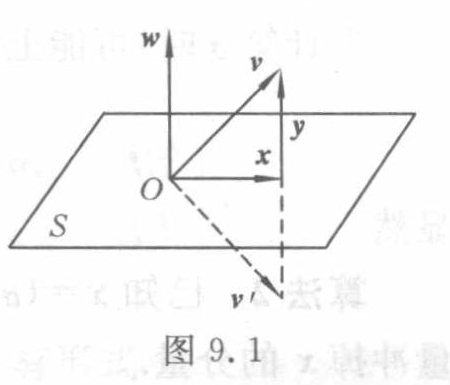
\includegraphics[width=0.85\linewidth,height=\textheight,keepaspectratio,alt={图 9.1，初等反射阵的几何意义，原图裁切}]{../assets/ch09a/fig-9-1.png}

图 9.1（原图裁切）。图中符号为 \(w,\allowbreak v,\allowbreak x,\allowbreak y,\allowbreak O,\allowbreak S,\allowbreak v'\)。超平面 \(S\) 经过原点 \(O\)，\(w\) 为法向量；\(v=x+y\) 分解为平面内分量 \(x\) 与垂直分量 \(y\)，\(v'\) 位于平面另一侧，表示镜面反射所得 \(x-y\)。原图用虚线连接 \(O\)、\(v'\) 端点及垂直分量方向。

初等反射阵在计算上的意义是它能用来约化矩阵，例如设向量 \(a\ne0\)，可选择一初等反射阵 \(H\) 使 \(H_a=\sigma e_1\)。这种约化矩阵的方法称为 Householder 方法。为此给出下面定理。

\textbf{定理 9.12} 设 \(x,y\) 为两个不相等的 \(n\) 维向量，\(\|x\|_2=\|y\|_2\)，则存在一个初等反射阵 \(H\)，使 \(Hx=y\)。

\textbf{证明} 令 \(w=\dfrac{x-y}{\|x-y\|_2}\)，则得到一个初等反射阵

\[
H=I-2ww^{\mathrm T}=I-2\frac{(x-y)}{\|x-y\|_2^2}(x^{\mathrm T}-y^{\mathrm T}),
\]

而且

\[
Hx=x-2\frac{x-y}{\|x-y\|_2^2}(x^{\mathrm T}-y^{\mathrm T})x=x-2\frac{(x-y)(x^{\mathrm T}x-y^{\mathrm T}x)}{\|x-y\|_2^2},
\]

因为

\[
\|x-y\|_2^2=(x-y)^{\mathrm T}(x-y)=2(x^{\mathrm T}x-y^{\mathrm T}x),
\]

所以

\[
Hx=x-(x-y)=y.
\]

易知，\(w=\dfrac{x-y}{\|x-y\|_2}\) 是使 \(Hx=y\) 成立的唯一长度等于 1 的向量（不计符号）。

\textbf{推论} 设向量 \(x\in\mathbf R^n\ (x\ne0)\)，\(\sigma=\pm\|x\|_2\)，且 \(x\ne-\sigma e_1\)，则存在一个初等反射阵

\[
H=I-2\frac{uu^{\mathrm T}}{\|u\|_2^2}\equiv I-\rho^{-1}uu^{\mathrm T},
\]

使 \(Hx=-\sigma e_1\)，其中 \(u=x+\sigma e_1\)，\(\rho=\|u\|_2^2/2\)。

设

\[
x=(\alpha_1,\alpha_2,\cdots,\alpha_n)^{\mathrm T}\ne0,\quad u=(u_1,u_2,\cdots,u_n)^{\mathrm T},
\]

\begin{quote}
\textbf{校注（agent 补充，ch09a-E008）} 在``可选择一初等反射阵 \(H\) 使''后，原图把 \(a\) 印在 \(H\) 的下标位置，故照录为 \(H_a=\sigma e_1\)。依本段语义及随后定理的矩阵作用，应为乘积 \(Ha=\sigma e_1\)；疑为原书排版错误。见\href{../assets/ch09a/review-p244-Ha.png}{放大原式}。
\end{quote}

\href{../../source-images/pdf-245.jpeg}{原页图像}

则

\[
u=(\alpha_1+\sigma,\alpha_2,\cdots,\alpha_n)^{\mathrm T},
\]

\[
\rho=\frac12\|u\|_2^2=\frac12\left[(\alpha_1+\sigma)^2+\alpha_2^2+\cdots+\alpha_n^2\right]=\sigma(\sigma+\alpha_1).
\]

如果 \(\sigma\) 和 \(\alpha_1\) 异号，那么计算 \(\alpha_1+\sigma\) 时有效数字可能损失，取 \(\sigma\) 和 \(\alpha_1\) 有相同的符号，即取

\[
\sigma=\operatorname{sgn}(\alpha_1)\|x\|_2.
\]

\textbf{算法 1} 已知向量 \(x=(\alpha_1,\alpha_2,\cdots,\alpha_n)^{\mathrm T}\ne0\)，本算法算出 \(\sigma,\rho\) 及 \(u\)，使 \((I-\rho^{-1}uu^{\mathrm T})x=-\sigma e_1\)，\(u\) 的分量冲掉 \(x\) 的分量。

\textbf{步 1} 计算 \(\sigma=\operatorname{sgn}(\alpha_1)\left(\displaystyle\sum_{i=1}^n\alpha_i^2\right)^{\frac12}\)。

\textbf{步 2} \(\alpha_1\to u_1=\alpha_1+\sigma\)。

\textbf{步 3} \(\rho=\sigma u_1\)。

在计算 \(\sigma\) 时，可能上溢或下溢。为了避免溢出，将 \(x\) 规范化

\[
\eta=\max_i|\alpha_i|,\quad x'=\frac{x}{\eta},
\]

显然

\[
\sigma'=\sigma/\eta,\quad H'=H.
\]

\textbf{算法 2} 已知 \(x=(\alpha_1,\alpha_2,\cdots,\alpha_n)^{\mathrm T}\ne0\)，本算法算出 \(H\) 及 \(\sigma\) 使 \(Hx=-\sigma e_1\)，\(u\) 的分量冲掉 \(x\) 的分量。

\textbf{步 1} \(\eta=\max_i|\alpha_i|\)。

\textbf{步 2} \(\alpha_i\leftarrow u_i=\dfrac{\alpha_i}{\eta}\quad(i=1,2,\cdots,n)\)。

\textbf{步 3} \(\sigma=\operatorname{sgn}(u_1)\left(\displaystyle\sum_{i=1}^nu_i^2\right)^{\frac12}\)。

\textbf{步 4} \(u_1\leftarrow u_1+\sigma\)。

\textbf{步 5} \(\rho=\sigma u_1\)。

\textbf{步 6} \(\sigma\leftarrow\eta\sigma\)。

关于 \(HA\) 的计算，设 \(A=(a_1,a_2,\cdots,a_n)\)，其中 \(a_i\) 为 \(A\) 的第 \(i\) 列向量，则

\[
HA=(Ha_1,Ha_2,\cdots,Ha_n),
\]

因此计算 \(HA\) 就是要计算

\[
Ha_i=(I-\rho^{-1}uu^{\mathrm T})a_i=a_i-(\rho^{-1}u^{\mathrm T}a_i)u\quad(i=1,2,\cdots,n).
\]

于是计算 \(Ha_i\) 只需要计算两向量的数量积和两向量的加法即可，且计算 \(HA\) 共需要 \(2n^2\) 次乘法运算。

\subsubsection{9.3.2 用正交相似变换约化矩阵}\label{ux7528ux6b63ux4ea4ux76f8ux4f3cux53d8ux6362ux7ea6ux5316ux77e9ux9635}

下面考虑用初等反射阵来正交相似约化一般矩阵和对称矩阵。设

\href{../../source-images/pdf-246.jpeg}{原页图像}

\[
A=\left(\begin{array}{c|ccc}
a_{11}&a_{12}&\cdots&a_{1n}\\\hline
a_{21}&a_{22}&\cdots&a_{2n}\\
\vdots&\vdots&&\vdots\\
a_{n1}&a_{n2}&\cdots&a_{nn}
\end{array}\right)
\equiv\begin{pmatrix}
a_{11}&A_{12}^{(1)}\\
a_{21}^{(1)}&A_{22}^{(1)}
\end{pmatrix},
\]

\textbf{步 1} 不妨设 \(a_{21}^{(1)}\ne0\)，否则这一步不需约化，选择初等反射阵 \(R_1\) 使 \(R_1a_{21}^{(1)}=-\sigma_1e_1\)，其中

\[
\left\{
\begin{aligned}
\sigma_1&=\operatorname{sgn}(a_{21})\left(\sum_{i=2}^na_{i1}^2\right)^{\frac12},\\
u_1&=a_{21}^{(1)}+\sigma_1e_1,\\
\rho_1&=\frac12\|u_1\|_2^2=\sigma_1(\sigma_1+a_{21}),\\
R_1&=I-\rho_1^{-1}u_1u_1^{\mathrm T}.
\end{aligned}
\right.
\tag{9.3.1}
\]

令 \(U_1=\begin{pmatrix}I&0\\0&R_1\end{pmatrix}\)，则

\[
A_2=U_1A_1U_1=\begin{pmatrix}
a_{11}&A_{21}^{(1)}R_1\\
R_1a_{21}^{(1)}&R_1A_{22}^{(1)}R_1
\end{pmatrix}
\equiv\begin{pmatrix}
A_{11}^{(2)}&a_{12}^{(2)}&A_{13}^{(2)}\\
O&a_{22}^{(2)}&A_{23}^{(2)}
\end{pmatrix},
\]

其中 \(A_{11}^{(2)}\in\mathbf R^{2\times1},\allowbreak \quad a_{22}^{(2)}\in\mathbf R^{n-2},\allowbreak \quad A_{23}^{(2)}\in\mathbf R^{(n-2)\times(n-2)}\)。

\textbf{步 \(k\)} 设对 \(A\) 已进行了第 \(k-1\) 步正交相似约化，即 \(A_k\) 有形式

\[
\begin{aligned}
A_k&=U_{k-1}A_{k-1}U_{k-1}\\
&=\left(\begin{array}{ccc|c|ccc}
a_{11}&a_{12}^{(2)}&\cdots&a_{1k}^{(k)}&a_{1,k+1}^{(k)}&\cdots&a_{1n}^{(k)}\\
-\sigma_1&a_{22}^{(2)}&\cdots&a_{2k}^{(k)}&a_{2,k+1}^{(k)}&\cdots&a_{2n}^{(k)}\\
&\ddots&\ddots&\vdots&\vdots&&\vdots\\
&&-\sigma_{k-1}&a_{kk}^{(k)}&a_{k,k+1}^{(k)}&\cdots&a_{k,n}^{(k)}\\\hline
&&&a_{k+1,k}^{(k)}&a_{k+1,k+1}^{(k)}&\cdots&a_{k+1,n}^{(k)}\\
&&&\vdots&\vdots&&\vdots\\
&&&a_{nk}^{(k)}&a_{n,k+1}^{(k)}&\cdots&a_{nn}^{(k)}
\end{array}\right)\\
&\equiv\begin{pmatrix}
A_{11}^{(k)}&a_{12}^{(k)}&A_{13}^{(k)}\\
O&a_{22}^{(k)}&A_{23}^{(k)}
\end{pmatrix},
\end{aligned}
\]

其中 \(A_{11}^{(k)}\in\mathbf R^{k\times(k-1)},\allowbreak \quad a_{22}^{(k)}\in\mathbf R^{n-k},\allowbreak \quad A_{23}^{(k)}\in\mathbf R^{(n-k)\times(n-k)}\)。

设 \(a_{22}^{(k)}\ne0\)，选择初等反射阵 \(R_k\)，使 \(R_ka_{22}^{(k)}=-\sigma_ke_1\)，其中

\[
\left\{
\begin{aligned}
\sigma_k&=\operatorname{sgn}(a_{k+1,k}^{(k)})\left(\sum_{i=k+1}^na_{ik}^2\right)^{\frac12},\\
u_k&=a_{22}^{(k)}+\sigma_ke_1,\\
\rho_k&=\frac12\|u_k\|_2^2=\sigma_k(\sigma_k+a_{k+1,n}^{(k)}),\\
R_k&=I-\rho_k^{-1}u_ku_k^{\mathrm T}.
\end{aligned}
\right.
\tag{9.3.2}
\]

\begin{quote}
\textbf{校注（agent 补充，ch09a-E009）} 本页 \(A_2\) 的二阶分块表达式右上块原印 \(A_{21}^{(1)}R_1\)，已照录。由页首定义的右上块 \(A_{12}^{(1)}\) 和 \(U_1\) 的分块乘法，此处应为 \(A_{12}^{(1)}R_1\)。见\href{../assets/ch09a/review-p246-initial-partition.png}{页首分块}和\href{../assets/ch09a/review-p246-A-2.png}{放大原式}。

\textbf{校注（agent 补充，ch09a-E010）} 式（9.3.2）原图 \(\sigma_k\) 求和内为 \(a_{ik}^2\)，未印迭代上标；\(\rho_k\) 最后一个矩阵元为 \(a_{k+1,n}^{(k)}\)，均照录。由本页 \(a_{22}^{(k)}=(a_{k+1,k}^{(k)},\ldots,a_{nk}^{(k)})^{\mathrm T}\) 和 \(u_k=a_{22}^{(k)}+\sigma_ke_1\)，求和应使用当前列元素 \((a_{ik}^{(k)})^2\)，而范数平方恒等式给出 \(\rho_k=\sigma_k(\sigma_k+a_{k+1,k}^{(k)})\)。故前者疑漏迭代上标，后者列下标疑将 \(k\) 印成 \(n\)。见\href{../assets/ch09a/review-p246-9-3-2.png}{放大原式}。
\end{quote}

\href{../../source-images/pdf-247.jpeg}{原页}

设 \(U_k=\begin{pmatrix}I&O\\O&R_k\end{pmatrix}\)，则

\[
A_{k+1}=U_kA_kU_k=
\begin{pmatrix}
A_{11}^{(k)}&a_{12}^{(k)}&A_{13}^{(k)}R_k\\
O&R_ka_{22}^{(k)}&R_kA_{23}^{(k)}R_k
\end{pmatrix}
=
\begin{pmatrix}
A_{11}^{(k)}&a_{12}^{(k)}&A_{13}^{(k)}R_k\\
O&-\sigma_ke_1&R_kA_{23}^{(k)}R_k
\end{pmatrix}.
\tag{9.3.3}
\]

由式（9.3.3）知，\(A_{k+1}\) 的左上角 \(k+1\) 阶子阵为上 Hessenberg 阵，从而约化又进了一步，重复这过程，直到

\[
U_{n-2}\cdots U_2U_1AU_1U_2\cdots U_{n-2}
=\begin{pmatrix}
a_{11}&\times&\times&\cdots&\times\\
-\sigma_1&a_{22}^{(2)}&\times&\cdots&\times\\
&-\sigma_2&a_{33}^{(3)}&\ddots&\vdots\\
&&\ddots&\ddots&\times\\
&&&-\sigma_{n-1}&a_{nn}^{(n-1)}
\end{pmatrix}=A_{n-1}.
\]

总结上述讨论，有如下定理。

\textbf{定理 9.13}　如果 \(A\in\mathbb R^{n\times n}\)，则存在初等反射阵 \(U_1,U_2,\cdots,U_{n-2}\)，使

\[
U_{n-2}\cdots U_2U_1AU_1U_2\cdots U_{n-2}=C\quad\text{（上 Hessenberg 阵）}.
\]

在 \(A_k\to A_{k+1}=U_kA_kU_k\) 的进一步约化中，需要计算 \(R_k\) 和 \(A_{13}^{(k)}R_k\)，\(R_kA_{23}^{(k)}R_k\)。用初等反射阵正交相似约化 \(A\) 为上 Hessenberg 阵，大约需要 \(\dfrac53n^3\) 次乘法运算。

由于 \(U_k\) 都是正交阵，所以 \(A_1\sim A_2\sim\cdots\sim A_{n-1}\)。求 \(A\) 的特征值问题，就转化为求上 Hessenberg 阵 \(C\) 的特征值问题。由定理 9.13，记 \(P=U_{n-2}\cdots U_2U_1\)，则

\[
PAP^{\mathrm T}=C.
\]

设 \(y\) 是 \(C\) 的对应特征值 \(\lambda\) 的特征向量，则 \(P^{\mathrm T}y\) 为 \(A\) 的对应特征值 \(\lambda\) 的特征向量，且

\[
P^{\mathrm T}y=U_1U_2\cdots U_{n-2}y
=(I-\lambda_1^{-1}u_1u_1^{\mathrm T})\cdots(I-\lambda_{n-2}^{-1}u_{n-2}u_{n-2}^{\mathrm T})y.
\]

\textbf{定理 9.14}　如果 \(A\in\mathbb R^{n\times n}\) 为对称阵，则存在初等反射阵 \(U_1,U_2,\cdots,U_{n-2}\)，使

\[
U_{n-2}\cdots U_2U_1AU_1U_2\cdots U_{n-2}=A_{n-1}
=\begin{pmatrix}
c_1&b_1&&&\\
b_1&c_2&b_2&&\\
&\ddots&\ddots&\ddots&\\
&&b_{n-2}&c_{n-1}&b_{n-1}\\
&&&b_{n-1}&c_n
\end{pmatrix}\equiv C.
\]

\textbf{证明}　由定理 9.13，存在初等反射阵 \(U_1,U_2,\cdots,U_{n-2}\)，使 \(A_{n-1}\) 为上 Hessenberg 阵，但 \(A_{n-1}\) 又为对称阵，因此 \(A_{n-1}\) 为对称三对角阵。

由上面讨论可知，在由 \(A_k\to A_{k+1}=U_kA_kU_k\) 一步计算过程中，只需计算 \(R_k\) 和 \(R_kA_{23}^{(k)}R_k\)。由于 \(A\) 的对称性，故只需计算 \(R_kA_{23}^{(k)}R_k\) 的对角线下面的元素。注意到

\[
R_kA_{23}^{(k)}R_k=(I-\rho_k^{-1}u_ku_k^{\mathrm T})(A_{23}^{(k)}-\rho_k^{-1}A_{23}^{(k)}u_ku_k^{\mathrm T}),
\]

\begin{quote}
校注（agent 补充）：本页 \(P^{\mathrm T}y\) 展开式原印为 \(\lambda_1^{-1}\)、\(\lambda_{n-2}^{-1}\)，而同页下方及次页初等反射阵的归一化因子使用 \(\rho_k^{-1}\)。此处保留原印 \(\lambda\)，记为疑似原书符号不一致。
\end{quote}

\href{../../source-images/pdf-248.jpeg}{原页}

引进记号

\[
r_k=\rho_k^{-1}A_{23}^{(k)}u_k,\qquad
 t_k=r_k-\frac{\rho_k^{-1}}2(u_k^{\mathrm T}r_k)u_k,
\]

则

\[
R_kA_{23}^{(k)}R_k=A_{23}^{(k)}-u_kt_k^{\mathrm T}-t_ku_k^{\mathrm T}
\quad(i=k+1,\cdots,n;\ j=k+1,\cdots,i).
\]

\textbf{算法 3}　正交相似约化对称阵为对称三对角阵。设 \(A\in\mathbb R^{n\times n}\) 是对称阵，本算法确定初等反射阵 \(U_1,U_2,\cdots,U_{n-2}\)，使 \(U_{n-2}\cdots U_1AU_1\cdots U_{n-2}=C\)（对称三对角阵），\(C\) 的对角元 \(c_i\) 存放在单元 \(c_1,c_2,\cdots,c_n\) 中，\(C\) 的非对角元 \(b_i\) 存放在单元 \(b_1,b_2,\cdots,b_{n-1}\) 中。单元 \(b_1,b_2,\cdots,b_n\) 最初可用来存放 \(r_k\) 及 \(t_k\) 的分量，确定 \(U_k\) 的向量 \(u_k\) 的分量 \(u_{k+1,k},\cdots,u_{nk}\)，存放在 \(A\) 的相应位置。\(\rho_k\) 冲掉 \(a_{kk}\)。约化 \(A\) 的结果冲掉 \(A\)，数组 \(A\) 的上部元素不变。如果步 \(k\) 不需要变换，则置 \(\rho_k\) 为零。

对于 \(k=1,2,\cdots,n-2\)，做到 \(L\)。

\textbf{步 1}　\(c_k=a_{kk}\)。

\textbf{步 2}　确定变换：

（1）计算 \(\eta=\max\limits_{k+1\leq i\leq n}|a_{ik}|\)；

（2）如果 \(\eta=0\)，则

\[
\begin{cases}
a_{kk}\to\rho_k=0,\\
b_k\to0,\\
\text{转 }L,\text{否则继续};
\end{cases}
\]

（3）计算 \(a_{ik}\leftarrow u_{ik}=a_{ik}/\eta\quad(i=k+1,\cdots,n)\)；

（4）\(\sigma=\operatorname{sgn}(u_{k+1,k})\sqrt{u_{k+1,k}^2+\cdots+u_{nk}^2}\)；

（5）\(u_{k+1,k}\leftarrow u_{k+1,k}+\sigma\)；

（6）\(a_{kk}\leftarrow\rho_k=\sigma u_{k+1,k}\)；

（7）\(b_k\leftarrow-\sigma\eta\)。

\textbf{步 3}　应用变换：

（1）\(\sigma=0\)；

（2）计算 \(A_{23}^{(k)}u_k\) 及 \(u_k^{\mathrm T}r_k\)，对于 \(i=k+1,\cdots,n\)，做

\[
\begin{cases}
b_i\leftarrow s=\displaystyle\sum_{j=k+1}^{n}a_{ij}u_{jk}+\displaystyle\sum_{j=i+1}^{n}a_{ji}u_{jk},\\
\sigma\leftarrow\sigma+su_{ik};
\end{cases}
\]

（3）计算 \(t_k\)

\[
b_i\leftarrow\rho_k^{-1}\left(b_i-\rho_k^{-1}\frac\sigma2u_{ik}\right)
\quad(i=k+1,\cdots,n);
\]

（4）计算 \(R_kA_{23}^{(k)}R_k\)

对于 \(i=k+1,\allowbreak k+2,\allowbreak \cdots,\allowbreak n;\ j=k+1,\allowbreak \cdots,\allowbreak i\)，做 \(a_{ij}\leftarrow a_{ij}-u_{ik}b_j-b_iu_{jk}\)。

\(L\)：继续循环。

对于 \(k=n-1\)，有

\[
c_{n-1}\leftarrow a_{n-1,n-1},\qquad c_n\leftarrow a_{nn},\qquad b_{n-1}\leftarrow a_{n,n-1}.
\]

\begin{quote}
校注（agent 补充）：算法 3 步 3（2）第一个求和上限原印为 \(n\)。按只存储、更新下三角部分的算法结构，该上限疑应为 \(i\)，否则 \(j>i\) 的项与第二个求和重叠，且会读入未更新的上三角元素。正文保留原印，列为疑似原书错误。
\end{quote}

\href{../../source-images/pdf-249.jpeg}{原页}

将对称阵 \(A\) 用初等反射阵正交相似约化为对称三对角阵约需做 \(\dfrac23n^3\) 次乘法运算。

用正交矩阵进行约化，有一些特点，如构造的 \(U_k\) 容易求逆，且 \(U_k\) 的元素数量级不大，因此这个算法是十分稳定的。

\textbf{例 9.5}　用 Householder 方法将下述矩阵化为上 Hessenberg 阵

\[
A_1=A=\begin{pmatrix}-4&-3&-7\\2&3&2\\4&2&7\end{pmatrix}.
\]

\textbf{解}　（1）对于 \(k=1\)，确定变换 \(U_1=\begin{pmatrix}1&\begin{matrix}0&0\end{matrix}\\\begin{matrix}0\\0\end{matrix}&R_1\end{pmatrix}\)，\(a_{21}^{(1)}=\begin{pmatrix}2\\4\end{pmatrix}\)，其中 \(R_1\) 为初等反射阵且使

\[
R_1a_{21}^{(1)}=-\sigma_1\begin{pmatrix}1\\0\end{pmatrix},\qquad
\sigma_1=\|a_{21}^{(1)}\|_2=\sqrt{20}\approx4.472\,136,
\]

\[
u_1=a_{21}^{(1)}+\sigma_1\rho_1=\begin{pmatrix}2+\sqrt{20}\\4\end{pmatrix}
\approx\begin{pmatrix}6.472\,136\\4\end{pmatrix},
\]

\[
\rho_1=\sigma_1(\sigma_1+a_{21})=\sqrt{20}(\sqrt{20}+2)\approx28.944\,27,\qquad
R_1=I-\rho_1^{-1}u_1u_1^{\mathrm T}.
\]

（2）计算 \(R_1A_{22}^{(1)}\)。记

\[
A_{22}^{(1)}=\begin{pmatrix}3&2\\2&7\end{pmatrix}\equiv(a_1,a_2),
\]

于是

\[
R_1A_{22}^{(1)}=(R_1a_1,R_1a_2)
=\begin{pmatrix}-3.130\,496&-7.155\,419\\-1.788\,855&1.341\,640\end{pmatrix},
\]

其中

\[
R_1a_i=(I-\rho_1^{-1}u_1u_1^{\mathrm T})a_i
=a_i-(\rho_1^{-1}u_1^{\mathrm T}a_i)u_1\quad(i=1,2).
\]

（3）计算 \(A_{12}^{(1)}R_1\) 及 \((R_1A_{22}^{(1)})R_1\)，即计算

\[
\begin{pmatrix}A_{12}^{(1)}\\(R_1A_{22}^{(1)})\end{pmatrix}R_1
\equiv\begin{pmatrix}b_1^{\mathrm T}\\b_2^{\mathrm T}\\b_3^{\mathrm T}\end{pmatrix}R_1
=\begin{pmatrix}b_1^{\mathrm T}R_1\\b_2^{\mathrm T}R_1\\b_3^{\mathrm T}R_1\end{pmatrix}
=\begin{pmatrix}
7.602\,634&-0.447\,212\\
7.800\,003&-0.399\,999\\
-0.399\,999&2.200\,000
\end{pmatrix},
\]

其中

\[
b_i^{\mathrm T}R_1=b_i^{\mathrm T}-(\rho_1^{-1}b_i^{\mathrm T}u_1)u_1^{\mathrm T}
\quad(i=1,2,3).
\]

（4）计算 \(A_2=U_1A_1U_1\)。

\[
A_2=\begin{pmatrix}-4&A_{12}^{(1)}R_1\\
\begin{matrix}-\sigma_1\\0\end{matrix}&R_1A_{22}^{(1)}R_1
\end{pmatrix}
=\begin{pmatrix}
-4&7.602\,634&-0.447\,212\\
-4.472\,136&7.800\,003&-0.399\,999\\
0&-0.399\,999&2.200\,000
\end{pmatrix}
\]

为上 Hessenberg 阵。

\begin{quote}
校注（agent 补充）：例 9.5（1）原印 \(u_1=a_{21}^{(1)}+\sigma_1\rho_1\) 中的 \(\rho_1\) 已经由放大原图确认。结合紧随的列向量以及同段将 \(\rho_1\) 定义为标量的公式，这里疑应为第一单位向量 \(e_1\)；正文保留原印。
\end{quote}

\href{../../source-images/pdf-250.jpeg}{原页}

\subsection{9.4 QR 算法}\label{qr-ux7b97ux6cd5}

\subsubsection{9.4.1 引言}\label{ux5f15ux8a00-2}

Rutishauser（在 1958 年）利用矩阵的三角分解提出了计算矩阵特征值的 LR 算法，Francis（在 1961 年、1962 年）利用矩阵的 QR 分解建立了计算矩阵特征值的 QR 方法。

QR 方法是一种变换方法，是计算一般矩阵（中小型矩阵）全部特征值问题的最有效的方法之一。目前，QR 方法主要用来计算：（1）上 Hessenberg 阵的全部特征值问题，（2）对称三对角阵的全部特征值问题。QR 方法具有收敛快、算法稳定等特点。

对于一般矩阵 \(A\in\mathbb R^{n\times n}\)（或对称阵），首先用 Householder 方法将 \(A\) 化为上 Hessenberg 阵 \(B\)（或对称三对角阵），然后再用 QR 方法计算 \(B\) 的全部特征值问题。

事实上，除了可以用 Householder 法约化矩阵外，还可考虑用如下形式的平面旋转矩阵来约化：

\[
P_{ij}=\left(\begin{array}{*{11}{c}}
1&&&&&&&&&&\\
&\ddots&&&&&&&&&\\
&&1&&&&&&&&\\
&&&c&&&&s&&&\\
&&&&1&&&&&&\\
&&&&&\ddots&&&&&\\
&&&&&&1&&&&\\
&&&-s&&&&c&&&\\
&&&&&&&&1&&\\
&&&&&&&&&\ddots&\\
&&&&&&&&&&1
\end{array}\right),
\tag{9.4.1}
\]

矩阵原图标注：\(c,-s\) 所在列为``第 \(i\) 列''，\(s,c\) 所在列为``第 \(j\) 列''；\(c,s\) 所在行为``第 \(i\) 行''，\(-s,c\) 所在行为``第 \(j\) 行''。其中 \(c=\cos\theta\)，\(s=\sin\theta\)。

下面是用这种矩阵约化矩阵的一些结论。

\textbf{引理 1}　设 \(x=(\alpha_1,\allowbreak \alpha_2,\allowbreak \cdots,\allowbreak \alpha_i,\allowbreak \cdots,\allowbreak \alpha_j,\allowbreak \cdots,\allowbreak \alpha_n)^{\mathrm T}\)，其中 \(\alpha_i,\alpha_j\) 不全为零，则可选一平面旋转矩阵 \(P_{ij}\) 使 \(P_{ij}x=y\equiv(\alpha_1,\allowbreak \alpha_2,\allowbreak \cdots,\allowbreak \alpha_i^{(1)},\allowbreak \cdots,\allowbreak \alpha_j^{(1)},\allowbreak \cdots,\allowbreak \alpha_n)^{\mathrm T}\)，其中

\[
\alpha_i^{(1)}=\sqrt{\alpha_i^2+\alpha_j^2},
\tag{9.4.2}
\]

\[
\alpha_j^{(1)}=0,
\tag{9.4.3}
\]

\[
\begin{cases}
c=\alpha_i/\sqrt{\alpha_i^2+\alpha_j^2},\\
s=\alpha_j/\sqrt{\alpha_i^2+\alpha_j^2}.
\end{cases}
\tag{9.4.4}
\]

\href{../../source-images/pdf-251.jpeg}{原页}

\textbf{证明}　事实上，\(P_{ij}x\) 只改变 \(x\) 的第 \(i\) 个及第 \(j\) 个元素，且有

\[
\alpha_i^{(1)}=c\alpha_i+s\alpha_j,\qquad
\alpha_j^{(1)}=-s\alpha_i+c\alpha_i,
\]

于是可选 \(P_{ij}\)，使 \(\alpha_j^{(1)}=-s\alpha_i+c\alpha_j=0\)，即按式（9.4.4）求 \(c,s\)，且有式（9.4.2）及式（9.4.3）。

用平面旋转阵进行左变换可产生一算法，设给定 \(x=\begin{pmatrix}\alpha\\\beta\end{pmatrix}\)，计算 \(c=\cos\theta\)，\(s=\sin\theta\)，\(v=\sqrt{\alpha^2+\beta^2}\)，使 \(P_{ij}x=\begin{pmatrix}c&s\\-s&c\end{pmatrix}\begin{pmatrix}\alpha\\\beta\end{pmatrix}=\begin{pmatrix}v\\0\end{pmatrix}\)，为了防止溢出，将 \(x\) 规范化，有

\[
\eta\equiv\|x\|_\infty=\max\{|\alpha|,|\beta|\}\ne0,\qquad
x'=x/\eta=\begin{pmatrix}\alpha/\eta\\\beta/\eta\end{pmatrix},
\]

于是

\[
\begin{cases}c'=c,\ s'=s,\\v'=v/\eta.\end{cases}
\]

\textbf{算法 1}　设 \(x=\begin{pmatrix}\alpha\\\beta\end{pmatrix}\)，本算法产生 \(c,s\) 及 \(v\)。

\textbf{步 1}　计算 \(\eta=\max\{|\alpha|,|\beta|\}\)。

\textbf{步 2}　如果 \(\eta=0\)，则 \(c\leftarrow1\)，\(s\leftarrow0\)，转步 8。

\textbf{步 3}　\(\alpha'=\alpha/\eta\)。

\textbf{步 4}　\(\beta'=\beta/\eta\)。

\textbf{步 5}　\(v'=\sqrt{\alpha'^2+\beta'^2}\)。

\textbf{步 6}　\(c=\alpha'/v'\)，\(s=\beta'/v'\)。

\textbf{步 7}　\(v=\eta v'\)。

\textbf{步 8}　计算终止。

\textbf{定理 9.15}　如果 \(A\) 为非奇异矩阵，则存在正交矩阵 \(P_1,P_2,\cdots,P_{n-1}\)（即一系列平面旋转矩阵）使

\[
P_{n-1},\cdots,P_2P_1A=\begin{pmatrix}
r_{11}&r_{12}&\cdots&r_{1n}\\
&r_{22}&\cdots&r_{2n}\\
&&\ddots&\vdots\\
&&&r_{nn}
\end{pmatrix}\equiv R,
\tag{9.4.5}
\]

且 \(r_{ii}>0\quad(i=1,2,\cdots,n-1)\)。

\textbf{证明}　由于 \(A\) 的第 1 列一定存在 \(a_{j1}\ne0\)，于是，如果 \(a_{j1}\ne0\ (j=2,3,\cdots,n)\)，应用算法 1，即存在平面旋转矩阵 \(P_{12},P_{13},\cdots,P_{1n}\)，使

\[
P_{1n}\cdots P_{13}P_{12}A=\begin{pmatrix}
r_{11}&a_{12}^{(2)}&\cdots&a_{1n}^{(2)}\\
0&a_{22}^{(2)}&\cdots&a_{2n}^{(2)}\\
\vdots&\vdots&&\vdots\\
0&a_{n2}^{(2)}&\cdots&a_{nn}^{(2)}
\end{pmatrix}\equiv A^{(2)},
\]

且记 \(P_{1n}\cdots P_{12}=P_1\)。同理，如果 \(a_{2j}^{(2)}\ne0\ (j=3,\cdots,n)\)，应用算法 1，存在平面旋转矩阵

\begin{quote}
校注（agent 补充）：引理 1 证明首式原印 \(\alpha_j^{(1)}=-s\alpha_i+c\alpha_i\)，下一行则为 \(-s\alpha_i+c\alpha_j\)。按矩阵乘法，首式末项疑应为 \(c\alpha_j\)；正文保留原印。

校注（agent 补充）：定理 9.15 证明末行原印 \(a_{2j}^{(2)}\ne0\)。该步旋转消去第 2 列下方元素，疑应为 \(a_{j2}^{(2)}\ne0\)；正文保留原印。

校注（agent 补充）：算法 1 步 2 的零向量分支只指定 \(c,s\) 后即终止，没有显式赋值 \(v\)。按开头的 \(v=\sqrt{\alpha^2+\beta^2}\)，此分支应有 \(v=0\)；原算法步骤保留。
\end{quote}

\href{../../source-images/pdf-252.jpeg}{原页}

\(P_{23},\cdots,P_{2n}\)（记 \(P_2=P_{2n}\cdots P_{23}\)），使

\[
P_2P_1A=\begin{pmatrix}
r_{11}&a_{12}^{(2)}&a_{13}^{(2)}&\cdots&a_{1n}^{(2)}\\
&r_{22}&a_{23}^{(3)}&\cdots&a_{2n}^{(3)}\\
&&a_{33}^{(3)}&\cdots&a_{3n}^{(3)}\\
&&\vdots&&\vdots\\
&&a_{n3}^{(3)}&\cdots&a_{nn}^{(3)}
\end{pmatrix}.
\]

重复上述过程，最后得到：存在正交阵 \(P_1,P_2,\cdots,P_{n-1}\)，使式（9.4.5）成立。

\textbf{定理 9.16（矩阵的 QR 分解）}　如果 \(A\in\mathbb R^{n\times n}\) 为非奇异矩阵，则 \(A\) 可分解为一正交阵 \(Q\) 与上三角阵 \(R\) 的乘积，即 \(A=QR\)，且当 \(R\) 对角元素都为正数时分解唯一。

\textbf{证明}　由定理 9.12，存在正交阵 \(P_1,P_2,\cdots,P_{n-1}\)，使

\[
P_{n-1}\cdots P_2P_1A=R
\tag{9.4.6}
\]

为上三角阵，记

\[
Q^{\mathrm T}=P_{n-1}\cdots P_2P_1,
\]

于是式（9.4.6）为 \(Q^{\mathrm T}A=R\)，即 \(A=QR\)，其中 \(Q=P_1^{\mathrm T}P_2^{\mathrm T}\cdots P_{n-1}^{\mathrm T}\) 为正交阵。

现证唯一性：设有 \(A=Q_1R_1=Q_2R_2\)，其中 \(R_1,R_2\) 为上三角阵（显然为非奇异阵）且对角元素都为正数，\(Q_1,Q_2\) 为正交阵。于是

\[
Q_2^{\mathrm T}Q_1=R_2R_1^{-1},
\tag{9.4.7}
\]

由式（9.4.7）知上三角阵 \(R_2R_1^{-1}\) 为正交阵，故 \(R_2R_1^{-1}\) 为对角阵，即

\[
R_2R_1^{-1}=D=\operatorname{diag}(d_1,d_2,\cdots,d_n).
\]

因为 \(R_2R_1^{-1}\) 是正交阵，所以 \(D^2=I\)，又因 \(R_1,R_2\) 对角元素都为正数，故 \(d_i>0\ (i=1,2,\cdots,n)\)，即 \(D=I\)。于是 \(R_2=R_1\)，由式（9.4.7）得到 \(Q_2=Q_1\)。

\subsubsection{9.4.2 QR 算法}\label{qr-ux7b97ux6cd5-1}

设 \(A=A_1=(a_{ij})\in\mathbb R^{n\times n}\)，且对 \(A\) 进行 QR 分解，即 \(A=QR\)，其中 \(R\) 为上三角阵，\(Q\) 为正交阵，于是可得到一新矩阵

\[
B=RQ=Q^{\mathrm T}AQ.
\]

显然，\(B\) 是由 \(A\) 经过正交相似变换得到，因此 \(B\) 与 \(A\) 特征值相同。再对 \(B\) 进行 QR 分解，又可得一新的矩阵，重复这过程可得到矩阵序列。

设 \(A=A_1\)，QR 分解，得 \(A_1=Q_1R_1\)，作矩阵 \(A_2=R_1Q_1=Q_1^{\mathrm T}A_1Q_1\)，\(\cdots\)，求得 \(A_k\) 后将 \(A_k\) 进行 QR 分解，得 \(A_k=Q_kR_k\)，作矩阵 \(A_{k+1}=R_kQ_k=Q_k^{\mathrm T}A_kQ_k\cdots\)。

QR 算法，就是利用矩阵的 QR 分解，按上述递推法则构造矩阵序列 \(\{A_k\}\) 的过程。只要 \(A\) 为非奇异矩阵，则由 QR 算法就完全确定 \(\{A_k\}\)。

\textbf{定理 9.17（基本 QR 方法）}　设 \(A=A_1\in\mathbb R^{n\times n}\)，QR 算法为

\[
\begin{cases}
A_k=Q_kR_k\quad(Q_k^{\mathrm T}Q_k=I,\ R_k\text{ 为上三角阵}),\\
A_{k+1}=R_kQ_k\quad(k=1,2,\cdots),
\end{cases}
\tag{9.4.8}
\]

\begin{quote}
校注（agent 补充）：定理 9.16 证明首句原印``由定理 9.12''，本段所需的平面旋转矩阵将 A 变成上三角阵的结论对应定理 9.15；原引用保留，列为疑似原书编号错误。
\end{quote}

\href{../../source-images/pdf-253.jpeg}{原页}

且记 \(\widetilde Q_k\equiv Q_1Q_2\cdots Q_k\)，\(\widetilde R_k\equiv R_k\cdots R_2R_1\)，则有

\(1^\circ\)　\(A_{k+1}\) 相似于 \(A_k\)，即 \(A_{k+1}=Q_k^{\mathrm T}A_kQ_k\)；

\(2^\circ\)　\(A_{k+1}=(Q_1Q_2\cdots Q_k)^{\mathrm T}A_1(Q_1Q_2\cdots Q_k)=\widetilde Q_k^{\mathrm T}A_1\widetilde Q_k\)；

\(3^\circ\)　\(A^k\) 的 QR 分解式为 \(A^k=\widetilde Q_k\widetilde R_k\)。

\textbf{证明}　结论 \(1^\circ\)、\(2^\circ\) 显然，现用归纳法证结论 \(3^\circ\)。显然，当 \(k=1\) 时有 \(A_1=\widetilde Q_1\widetilde R_1=Q_1R_1\)，设 \(A^{k-1}\) 有分解式 \(A^{k-1}=\widetilde Q_{k-1}\widetilde R_{k-1}\)，于是

\[
\begin{aligned}
\widetilde Q_k\widetilde R_k
&=Q_1Q_2\cdots(Q_kR_k)\cdots R_1
=Q_1Q_2\cdots Q_{k-1}A_kR_{k-1}\cdots R_1\\
&=\widetilde Q_{k-1}A_k\widetilde R_{k-1}
=A\widetilde Q_{k-1}\widetilde R_{k-1}=A^k
\quad\text{（因为 }A_k=\widetilde Q_{k-1}^{\mathrm T}A\widetilde Q_{k-1}\text{）}.
\end{aligned}
\]

由定理 9.13 知，将 \(A_k\) 进行 QR 分解，即将 \(A_k\) 用正交变换（左变换）化为上三角阵。

\[
Q_k^{\mathrm T}A_k=R_k,\qquad
A_{k+1}=Q_k^{\mathrm T}A_kQ_k=P_{n-1}\cdots P_2P_1A_kP_1^{\mathrm T}P_2^{\mathrm T}\cdots P_{n-1}^{\mathrm T},
\]

其中

\[
Q_k^{\mathrm T}=P_{n-1}\cdots P_2P_1.
\]

这就是说 \(A_{k+1}\) 可由 \(A_k\) 按下述方法求得：

（1）左变换 \(P_{n-1}\cdots P_2P_1A_k=R_k\)（上三角阵）；（2）右变换 \(R_kP_1^{\mathrm T}P_2^{\mathrm T}\cdots P_{n-1}^{\mathrm T}=A_{k+1}\)。

\textbf{引理 2}　设 \(M_k=Q_kR_k\)，其中 \(Q_k\) 为正交阵，\(R_k\) 为具有正对角元素的上三角阵，如果 \(M_k\to I\ (k\to\infty)\)，则 \(Q_k\to I\)，及 \(R_k\to I\ (k\to\infty)\)。

\textbf{证明}　设 \(R_k^{\mathrm T}R_k=M_k^{\mathrm T}M_k\to I\ (k\to\infty)\)，记 \(R_k=(r_{ij}^{(k)})\)，矩阵 \(R_k^{\mathrm T}R_k\) 第 1 行是

\[
r_{11}^{(k)}\cdot(r_{11}^{(k)},r_{12}^{(k)},\cdots,r_{1n}^{(k)}),
\]

因此有

\[
r_{11}^{(k)}\to1,\ r_{12}^{(k)}\to0,\ \cdots,\ r_{1n}^{(k)}\to0\quad(k\to\infty).
\tag{9.4.9}
\]

\(R_k^{\mathrm T}R_k\) 第 2 行是

\[
r_{12}^{(k)}\cdot(r_{11}^{(k)},r_{12}^{(k)},\cdots,r_{1n}^{(k)})
+r_{22}^{(k)}\cdot(0,r_{22}^{(k)},r_{23}^{(k)},\cdots,r_{2n}^{(k)}),
\]

利用式（9.4.9）的结果，则有

\[
r_{22}^{(k)}\to1,\ r_{23}^{(k)}\to0,\ \cdots,\ r_{2n}^{(k)}\to0\quad(k\to\infty).
\tag{9.4.10}
\]

对于 \(R_k^{\mathrm T}R_k\) 其他行同理可得，故 \(R_k\to I\ (k\to\infty)\)，且易知有 \(R_k^{-1}\to I\ (k\to\infty)\)，因此 \(Q_k=M_kR_k^{-1}\to I\ (k\to\infty)\)。

\textbf{定理 9.18（QR 方法的收敛性）}　设 \(A=(a_{ij})\in\mathbb R^{n\times n}\)，

\(1^\circ\) 如果 \(A\) 的特征值满足：\(|\lambda_1|>|\lambda_2|>\cdots>|\lambda_n|>0\)；

\(2^\circ\) \(A\) 有标准形 \(A=XDX^{-1}\) 其中 \(D=\operatorname{diag}(\lambda_1,\lambda_2,\cdots,\lambda_n)\)，且设 \(X^{-1}\) 有三角分解 \(X^{-1}=LU\)（\(L\) 为单位下三角阵，\(U\) 为上三角阵），则由 QR 算法产生的 \(\{A_k\}\) 本质上收敛于上三角阵，即

\[
A_k\xrightarrow{\text{本质上}}R=
\begin{pmatrix}
\lambda_1&\times&\cdots&\times\\
&\lambda_2&\ddots&\vdots\\
&&\ddots&\times\\
&&&\lambda_n
\end{pmatrix}\quad(k\to\infty)
\]

\begin{quote}
校注（agent 补充）：本页将 QR 分解引用为``定理 9.13''，而 PDF247 上定理 9.13 的结论是约化为上 Hessenberg 阵；本页所述左变换为上三角阵的结论见定理 9.15。保留原引用，列为疑似原书编号错误。
\end{quote}

\href{../../source-images/pdf-254.jpeg}{原页}

或

\[
a_{ii}^{(k)}\to\lambda_i\quad(k\to\infty),
\tag{9.4.11}
\]

当 \(i>j\) 时，

\[
a_{ij}^{(k)}\to0\quad(k\to\infty).
\tag{9.4.12}
\]

当 \(i<j\) 时，\(a_{ij}^{(k)}\) 极限不一定存在。

\textbf{证明}　由于 \(A_{k+1}=\widetilde Q_k^{\mathrm T}A_1\widetilde Q_k\) 且 \(\widetilde Q_k\) 为 \(A^k\) 的 QR 分解中的正交矩阵。下面来确定 \(\widetilde Q_k\) 的表达式，进而考虑 \(A_{k+1}\) 的极限情况。

由于 \(A\) 为非奇异矩阵，所以存在非奇异矩阵 \(X\) 使 \(X^{-1}AX=D\)，则

\[
A^k=XD^kX^{-1},
\tag{9.4.13}
\]

又有假设 \(X^{-1}=LU\)，于是式（9.4.13）为

\[
A^k=XD^kLU=X(D^kLD^{-k})D^kU.
\]

显然

\[
D^kLD^{-k}=I+E_k,
\]

其中

\[
E_k=\begin{pmatrix}
0&&&&\\
\left(\dfrac{\lambda_2}{\lambda_1}\right)^k l_{21}&0&&&\\
\left(\dfrac{\lambda_3}{\lambda_1}\right)^k l_{31}&\left(\dfrac{\lambda_3}{\lambda_2}\right)^k l_{32}&0&&\\
\vdots&\vdots&\ddots&\ddots&\\
\left(\dfrac{\lambda_n}{\lambda_1}\right)^k l_{n1}&\left(\dfrac{\lambda_n}{\lambda_2}\right)^k l_{n2}&\cdots&\left(\dfrac{\lambda_n}{\lambda_{n-1}}\right)^k l_{n,n-1}&0
\end{pmatrix}.
\]

由假设条件 \(|\lambda_i/\lambda_j|<1\)（当 \(i>j\) 时），则 \(E_k\to O\ (k\to\infty)\) 且

\[
\|E_k\|_\infty\leq c\max_{1\leq j\leq n-1}|\lambda_{j+1}/\lambda_j|^k
\quad(c\text{ 为正的常数},\ k\geq1).
\tag{9.4.14}
\]

显然矩阵 \(X\) 有 QR 分解：\(X=QR\)，其中 \(Q\) 为正交阵，\(R\) 为非奇异上三角阵。于是

\[
A^k=QR(I+E_k)D^kU=Q(I+RE_kR^{-1})RD^kU.
\tag{9.4.15}
\]

由于 \(R(I+E_k)\)（当 \(k\) 充分大时）为非奇异，则 \(I+RE_kR^{-1}\) 亦非奇异，于是 \((I+RE_kR^{-1})\) 有 QR 分解（要求 \(R_k\) 对角元素均为正）

\[
I+RE_kR^{-1}=Q_kR_k\quad\text{且}\quad Q_kR_k\to I\quad\text{（当 }k\to\infty\text{ 时）},
\]

由引理 2 有 \(Q_k\to I,R_k\to I\)（当 \(k\to\infty\) 时），由式（4.15）有

\[
A^k=(QQ_k)(R_kRD^kU),
\tag{9.4.16}
\]

式（9.4.16）为 \(A^k\) 的 QR 分解式，但 \(R_kRD^kU\)（为上三角阵）对角元素不一定大于零，现引入对角阵

\[
D_k=\operatorname{diag}(\pm1,\pm1,\cdots,\pm1),
\]

以便保证 \(D_k(R_kRD^kU)\) 对角元素都为正数。从而得到 \(A^k\) 的 QR 分解式

\[
A^k=(QQ_kD_k)(D_kR_kRD^kU),
\]

由 \(A^k\) 矩阵 QR 分解的唯一性得到

\[
\begin{cases}
\widetilde Q_k=QQ_kD_k,\\
\widetilde R_k=D_kR_kRD^kU,
\end{cases}
\tag{9.4.17}
\]

\begin{quote}
校注（agent 补充）：式（9.4.16）前原印``由式（4.15）有''，本页对应公式编号为（9.4.15）。正文保留原印编号。
\end{quote}

\href{../../source-images/pdf-255.jpeg}{原页}

从而

\[
A_{k+1}=\widetilde Q_k^{\mathrm T}A\widetilde Q_k
=D_kQ_k^{\mathrm T}(RDR^{-1})Q_kD_k
\quad\text{（注意 }Q^{\mathrm T}AQ=RDR^{-1}\text{）},
\]

其中

\[
R_0\equiv RDR^{-1}=\begin{pmatrix}
\lambda_1&\times&\cdots&\times\\
&\lambda_2&\ddots&\vdots\\
&&\ddots&\times\\
&&&\lambda_n
\end{pmatrix},
\]

于是

\[
A_{k+1}=g_k^{\mathrm T}R_0g_k,
\]

其中

\[
\begin{cases}
g_k=Q_kD_k,\\
R_0=RDR^{-1}\quad\text{（上三角阵）},\\
Q_k\to I\quad(k\to\infty),\\
D_k\text{ 为对角阵，其元素为 }+1\text{ 或 }-1.
\end{cases}
\]

由此即证得式（9.4.11）、式（9.4.12）。且收敛速度依赖于 \(Q_k\to I\) 收敛速度；即依赖于式（9.4.14）的界。

\textbf{定理 9.19}　如果对称阵 \(A\) 满足定理 9.18 条件，则由 QR 算法产生的 \(\{A_k\}\) 收敛于对角阵。

\textbf{证明}　由定理 9.18 即知。下面提一下关于 QR 算法收敛性的另一结果。

设 \(A\in\mathbb R^{n\times n}\)，如果 \(A\) 的等模特征值中只有实重特征值或多重复的共轭特征值，则由 QR 算法产生 \(\{A_k\}\) 本质收敛于分块上三角阵（对角块为一阶和二阶子块）且对角块每一个 \(2\times2\) 子块给出 \(A\) 的一对共轭复特征值，每一个对角子块给出 \(A\) 的实特征值，即

\[
A_k\to\begin{pmatrix}
\lambda_1&\times&\cdots&\times&\times\times&\cdots&\times\times\\
&\lambda_2&\ddots&\vdots&\vdots&&\vdots\\
&&\ddots&\times&\vdots&&\vdots\\
&&&\lambda_m&\times\times&\cdots&\times\times\\
&&&&B_l&\ddots&\vdots\\
&&&&&\ddots&\times\times\\
&&&&&&B_l
\end{pmatrix}.
\]

其中 \(m+2l=n\)，\(B_i\) 为 \(2\times2\) 子块给出 \(A\) 一对共轭特征值。

\subsubsection{9.4.3 带原点位移的 QR 方法}\label{ux5e26ux539fux70b9ux4f4dux79fbux7684-qr-ux65b9ux6cd5}

在定理 9.18 证明中进一步分析可知，\(a_{nn}^{(k)}\to\lambda_n\ (k\to\infty)\) 速度依赖于比值 \(r_n=|\lambda_n/\lambda_{n-1}|\)，当 \(r_n\) 很小时，收敛较快，如果 \(s\) 为 \(\lambda_n\) 一个估计，且对 \(A-sI\) 运用 QR 算法，则 \((n,n-1)\) 元素将以收敛因子 \(\left|\dfrac{\lambda_n-s}{\lambda_{n-1}-s}\right|\) 线性收敛于零，\((n,n)\) 元素将比在基本算法中收敛更快。

\begin{quote}
校注（agent 补充）：上方分块上三角阵中第一个二阶对角块原印为 \(B_l\)，与末块同名；放大字形确认后照录。按 \(m+2l=n\) 及顺序编号，第一个二阶块疑应为 \(B_1\)。
\end{quote}

\href{../../source-images/pdf-256.jpeg}{原页}

为此，为了加速收敛，选择数列 \(\{s_k\}\)，按下述方法构造矩阵序列 \(\{A_k\}\)，称为\textbf{带原点位移的 QR 算法}。

\textbf{步 1}　设 \(A=A_1\in\mathbb R^{n\times n}\)。

\textbf{步 2}　将 \(A_k-s_kI\) 进行 QR 分解，即 \(A_k-s_kI=Q_kR_k\)，\(k=1,2,\cdots\)。

\textbf{步 3}　构造新矩阵 \(A_{k+1}=R_kQ_k+s_kI=Q_k^{\mathrm T}A_kQ_k\)。

\textbf{步 4}　\(A_{k+1}=\widetilde Q_k^{\mathrm T}A\widetilde Q_k\)，其中 \(\widetilde Q_k=Q_1Q_2\cdots Q_k\)，\(\widetilde R_k=R_k\cdots R_2R_1\)。

\textbf{步 5}　矩阵 \((A-s_1I)(A-s_2I)\cdots(A-s_kI)\equiv\varphi(A)\) 有 QR 分解式 \(\varphi(A)=\widetilde Q_k\widetilde R_k\)。

\textbf{步 6}　带位移 QR 方法变换一步的计算：首先用正交变换（左变换）将 \(A_k-s_kI\) 化为上三角阵，即

\[
P_{n-1}\cdots P_2P_1(A_k-s_kI)=R_k,
\]

其中 \(Q_k^{\mathrm T}=P_{n-1}\cdots P_2P_1\) 为一系列平面旋转矩阵的乘积。于是

\[
A_{k+1}=P_{n-1}\cdots P_2P_1(A_k-s_kI)P_1^{\mathrm T}P_2^{\mathrm T}\cdots P_{n-1}^{\mathrm T}+s_kI.
\]

下面考虑用 QR 算法计算上 Hessenberg 阵特征值。

设

\[
A=A_1=\begin{pmatrix}
a_{11}&a_{12}&\cdots&a_{1n}\\
a_{21}&a_{22}&\cdots&a_{2n}\\
&\ddots&\ddots&\vdots\\
&&a_{n,n-1}&a_{nn}
\end{pmatrix},\quad A\in\mathbb R^{n\times n}.
\]

（1）左变换计算。选择平面旋转阵 \(P_{12},P_{23},\cdots,P_{n-1,n}\)，使

\[
P_{n-1,n}\cdots P_{23}P_{12}(A_1-s_1I)=R.
\]

首先

\[
a_{ii}\leftarrow a_{ii}-s_1\quad(i=1,2,\cdots,n).
\]

第一次左变换，选择平面旋转阵 \(P_{12}\)，使第 2 行第 1 列元素为零。

\[
P_{12}(A_1-s_1I)=\begin{pmatrix}
v_1&\begin{matrix}a_{12}^{(2)}&a_{13}^{(2)}&\cdots&a_{1n}^{(2)}\end{matrix}\\
&\boxed{\begin{matrix}
a_{22}^{(2)}&a_{23}^{(2)}&\cdots&a_{2n}^{(2)}\\
a_{32}&a_{33}&\cdots&a_{3n}\\
&\ddots&\ddots&\vdots\\
&&a_{n,n-1}&a_{nn}
\end{matrix}}
\end{pmatrix}.
\]

设已完成第 \(i-1\) 次左变换，则

\[
P_{i-1,i}\cdots P_{23}P_{12}(A_1-s_1I)
=\begin{pmatrix}
v_1&a_{12}^{(2)}&\cdots&\cdots&\begin{matrix}\cdots&\cdots&\cdots&a_{1n}^{(2)}\end{matrix}\\
&v_2&a_{23}^{(2)}&\cdots&\begin{matrix}\cdots&\cdots&\cdots&a_{2n}^{(2)}\end{matrix}\\
&&\ddots&\ddots&\begin{matrix}&&&\vdots\end{matrix}\\
&&&v_{i-1}&\begin{matrix}a_{i-1,i}^{(i-1)}&\cdots&\cdots&a_{i-1,n}^{(i-1)}\end{matrix}\\
&&&&\boxed{\begin{matrix}
a_{ii}^{(i)}&\cdots&\cdots&a_{in}^{(i)}\\
a_{i+1,i}&\ddots&&a_{i+1,n}\\
&\ddots&\ddots&\vdots\\
&&a_{n,n-1}&a_{nn}
\end{matrix}}
\end{pmatrix}.
\]

\href{../../source-images/pdf-257.jpeg}{原页}

现进行第 \(i\) 次左变换，选择 \(P_{i,i+1}\)（常数 \(c_i,s_i\)）及 \(v_k\) 使 \((i+1,i)\)---元素为零，则有

\[
P_{i,i+1}\cdots P_{23}P_{12}(A_1-s_1I)
=\begin{pmatrix}
v_1&\times&\cdots&\cdots&\begin{matrix}\cdots&\cdots&\times\end{matrix}\\
&v_2&\times&\cdots&\begin{matrix}\cdots&\cdots&\times\end{matrix}\\
&&\ddots&\ddots&\begin{matrix}&&\vdots\end{matrix}\\
&&&v_i&\begin{matrix}\times&\cdots&\times\end{matrix}\\
&&&&\boxed{\begin{matrix}
\times&\times&\cdots&\times\\
\times&\ddots&\ddots&\vdots\\
&\ddots&\ddots&\times\\
&&\times&\times
\end{matrix}}
\end{pmatrix},
\]

继续这过程，最后

\[
P_{n-1,n}\cdots P_{23}P_{12}(A_1-s_1I)=R\quad\text{（上三角阵）},
\]

其中 \(P_{i,i+1}\ (i=1,2,\cdots,n+1)\) 为平面旋转阵。

（2）右变换计算。计算 \(RP_{12}^{\mathrm T}P_{23}^{\mathrm T}\cdots P_{n-1,n}^{\mathrm T}\)，其中上三角阵 \(R\) 元素仍记作 \(a_{ij}\ (i\leq j)\)，于是

\[
RP_{12}^{\mathrm T}=\begin{pmatrix}
a_{11}^{(2)}&a_{12}^{(2)}&a_{13}&\cdots&a_{1n}\\
a_{21}^{(2)}&a_{22}^{(2)}&a_{23}&\cdots&a_{2n}\\
&&a_{33}&\cdots&a_{3n}\\
&&&\ddots&\vdots\\
&&&&a_{nn}
\end{pmatrix},
\]

\[
RP_{12}^{\mathrm T}P_{23}^{\mathrm T}=\begin{pmatrix}
a_{11}^{(2)}&a_{12}^{(3)}&a_{13}^{(3)}&a_{14}&\cdots\\
a_{21}^{(2)}&a_{22}^{(3)}&a_{23}^{(3)}&a_{24}&\cdots\\
&a_{32}^{(3)}&a_{33}^{(3)}&a_{34}&\cdots\\
&&a_{43}^{(3)}&a_{44}&\cdots\\
&&&\ddots&\ddots
\end{pmatrix}.
\]

继续这过程，最后

\[
RP_{12}^{\mathrm T}P_{23}^{\mathrm T}\cdots P_{n-1,n}^{\mathrm T}
=\begin{bmatrix}
\times&\times&\cdots&\cdots&\times\\
\times&\times&\cdots&\cdots&\times\\
&\times&\ddots&&\vdots\\
&&\ddots&\ddots&\vdots\\
&&&\times&\times
\end{bmatrix}\quad\text{（为上 Hessenberg 阵）},
\]

故 \(A_2=RP_{12}^{\mathrm T}P_{23}^{\mathrm T}\cdots P_{n-1,n}^{\mathrm T}+s_1I\) 为上 Hessenberg 阵。

由上面的构造可知，如果 \(A\) 为上 Hessenberg 阵，则用 QR 算法产生的 \(A_2,A_3,\cdots,A_k,\cdots\) 亦是上 Hessenberg 阵。显然，每一次左变换仅改变矩阵的两行，而每一次右变换仅改变矩阵的两列。为了节省存储量，左变换和右变换可以同时进行，例如

\[
\begin{aligned}
P_{23}P_{12}(A-s_1I)&\to P_{23}P_{12}(A-s_1I)P_{12}^{\mathrm T}
\to P_{34}P_{23}P_{12}(A-s_1I)P_{12}^{\mathrm T}\\
&\to P_{34}P_{23}P_{12}(A-s_1I)P_{12}^{\mathrm T}P_{23}^{\mathrm T}\to\cdots
\end{aligned}
\]

实际计算时，用不同位移 \(s_1,s_2,\cdots,s_k,\cdots\) 反复应用上述变换就产生一正交相似于上 Hessenberg 阵 \(A\) 的序列 \(\{A_k\}\)，如果选取 \(s_k=a_{nn}^{(k)}\)，那么当 \(a_{n,n-1}^{(k)}\) 充分小，\(A_k\) 有形式

\begin{quote}
校注（agent 补充）：本页开头第 \(i\) 次左变换原印``及 \(v_k\)''，对应矩阵对角位置为 \(v_i\)，疑为下标不一致；保留原印。

校注（agent 补充）：左变换最后一式之后原印 \(i=1,2,\cdots,n+1\)。因 \(P_{i,i+1}\) 作用于 \(n\) 阶矩阵，且乘积末项为 \(P_{n-1,n}\)，上限疑应为 \(n-1\)；保留原印。
\end{quote}

\href{../../source-images/pdf-258.jpeg}{原页}

\[
\left(\begin{array}{ccccc|c}
\times&\times&\times&\cdots&\times&\times\\
&\times&\times&\cdots&\times&\times\\
&&\ddots&\ddots&\vdots&\vdots\\
&&&\times&\times&\times\\\hline
&&&&&\lambda_n
\end{array}\right)_{n\times n}
\equiv\left(\begin{array}{c|c}
B&\begin{matrix}\times\\\times\\\vdots\\\times\end{matrix}\\\hline
O&\lambda_n
\end{array}\right),
\]

则数 \(\lambda_n=a_{nn}^{(k)}\) 为 \(A\) 的近似特征值。采用收缩方法，继续对 \(B\in\mathbb R^{(n-1)\times(n-1)}\) 应用 QR 算法，就可逐步求出 \(A\) 其余近似特征值。

判别 \(a_{n,n-1}^{(k)}\) 充分小的准则如下：

（1）\(|a_{n,n-1}^{(k)}|\leq\varepsilon\|A\|_\infty\)；

（2）或将 \(a_{n,n-1}^{(k)}\) 与相邻元素进行比较 \(|a_{n,n-1}^{(k)}|\leq\varepsilon\min(|a_{nn}^{(k)}|,|a_{n-1,n-1}^{(k)}|)\)，其中 \(\varepsilon=10^{-t}\)，\(t\) 是计算中有效数字的个数。

上述应用带位移的 QR 算法，可计算上 Hessenberg 阵 \(A\) 所有特征值，但不能计算 \(A\) 复特征值，因为上述 QR 算法是在实数中进行计算的，位移 \(s_k=a_{nn}\) 不能逼近一个复特征值。关于避免复数运算求上 Hessenberg 阵复特征值的 QR 算法------隐式位移的 QR 算法请参看有关文献。

一般来说位移 \(s_k\) 常用的选取方法有两种：

（1）选取 \(s_k=a_{nn}^{(k)}\)；

（2）选取 \(s_k\) 是 \(2\times2\) 矩阵 \(\begin{pmatrix}a_{n-1,n-1}^{(k)}&a_{n-1,n}^{(k)}\\a_{n,n-1}^{(k)}&a_{nn}^{(k)}\end{pmatrix}\)，特征值 \(\lambda\) 且 \(|a_{nn}^{(k)}-\lambda|\) 为最小（记 \(A_k=(a_{ij}^{(k)})\)）。

\textbf{例 9.6}　用 QR 方法计算对称三对角阵的全部特征值

\[
A=A_1=\begin{pmatrix}2&1&0\\1&3&1\\0&1&4\end{pmatrix}.
\]

\textbf{解}　采用第一种选位移方法，即选 \(s_k=a_{nn}^{(k)}\)。又 \(s_1=4\)。

\[
P_{23}P_{12}(A_1-s_1I)=R=\begin{pmatrix}
2.236\,1&-1.342&0.447\,2\\
&1.095\,4&-0.365\,1\\
&&0.816\,50
\end{pmatrix},
\]

\[
A_2=RP_{12}^{\mathrm T}P_{23}^{\mathrm T}+s_1I
=\begin{pmatrix}
1.400\,0&0.489\,9&0\\
0.489\,9&3.266\,7&0.745\,4\\
0&0.745\,4&4.333\,3
\end{pmatrix},
\]

\[
A_3=\begin{pmatrix}
1.291\,5&0.201\,7&0\\
0.201\,7&3.020\,2&0.272\,4\\
0&0.272\,4&4.688\,4
\end{pmatrix},\qquad
A_4=\begin{pmatrix}
1.273\,7&0.099\,3&0\\
0.099\,3&2.994\,3&0.007\,2\\
0&0.007\,2&4.732\,0
\end{pmatrix},
\]

\href{../../source-images/pdf-259.jpeg}{原页}

\[
A_5=\begin{pmatrix}
1.269\,4&0.049\,8&0\\
0.049\,8&2.998\,6&0\\
0&0&\boxed{4.732\,1}
\end{pmatrix},\qquad
\widetilde A_5=\begin{pmatrix}1.269\,4&0.049\,8\\0.049\,8&2.998\,6\end{pmatrix}.
\]

现在收缩，继续对 \(A_5\) 的子矩阵 \(\widetilde A_5\in\mathbb R^{2\times2}\) 进行变换，得到

\[
\widetilde A_6=P_{12}(\widetilde A_5-s_5I)P_{12}^{\mathrm T}+s_5I
=\begin{pmatrix}\boxed{1.268\,0}&-4\times10^{-5}\\-4\times10^{-5}&\boxed{3.000\,0}\end{pmatrix},
\]

故求得 \(A\) 近似特征值为

\[
\lambda_1\approx4.732\,1,\qquad\lambda_2\approx3.000\,0,\qquad\lambda_3\approx1.268\,0,
\]

且 \(A\) 的特征值是

\[
\lambda_1=3+\sqrt3\approx4.732\,1,\qquad\lambda_2=3.0,\qquad\lambda_3=3-\sqrt3\approx1.267\,9.
\]

\subsection{小结}\label{ux5c0fux7ed3}

本章介绍了计算一般矩阵主特征值及对应特征向量的迭代法（幂法），这种方法在计算过程中原始矩阵 \(A\) 始终不变。因此，这种方法适于求高阶稀疏矩阵的特征值问题。主特征值为复特征值情况可参看文献 {[}11{]}。

反幂法是计算矩阵特征向量的一个有效方法，主要用来计算 Hessenberg 阵或三对角阵对应于一个给定的近似特征值的特征向量。

本章还介绍了正交相似变换的方法，例如正交相似约化一般矩阵 \(A\) 为上 Hessenberg 阵的 Householder 方法，计算一般矩阵 \(A\) 全部特征值问题的 QR 方法，这些方法都是利用矩阵的正交相似变换约化矩阵 \(A\) 为某种简单形式，以期求 \(A\) 的特征值的方法。这种方法将破坏原始矩阵。QR 方法（与 Householder 方法结合使用）收敛快，精度高，是求任意实矩阵（中、小型）特征值问题的最有效的方法之一。对计算矩阵特征值问题有兴趣的读者可参看文献 {[}10{]}、{[}13{]}、{[}14{]}。

\subsection{习题}\label{ux4e60ux9898}

\textbf{1.} 用幂法计算下列矩阵的主特征值及对应的特征向量：

\[
\text{（1）}\ A_1=\begin{pmatrix}7&3&-2\\3&4&-1\\-2&-1&3\end{pmatrix};\qquad
\text{（2）}\ A_2=\begin{pmatrix}3&-4&3\\-4&6&3\\3&3&1\end{pmatrix},
\]

当特征值有三位小数稳定时迭代终止。

\textbf{2.} 方阵 \(T\) 分块形式为

\[
T=\begin{pmatrix}
T_{11}&T_{12}&\cdots&T_{1n}\\
&T_{22}&\cdots&T_{2n}\\
&&\ddots&\vdots\\
&&&T_{nn}
\end{pmatrix},
\]

其中 \(T_{ii}\ (i=1,2,\cdots,n)\) 为方阵，\(T\) 称为块上

\href{../../source-images/pdf-260.jpeg}{原页}

三角阵，如果对角块的阶数至多不超过 2，则称 \(T\) 为准三角形形式。用 \(\sigma(T)\) 记矩阵 \(T\) 的特征值集合，证明 \(\sigma(T)=\displaystyle\bigcup_{i=1}^{n}\sigma(T_{ii})\)。

\textbf{3.} 利用反幂法求矩阵 \(\begin{pmatrix}6&2&1\\2&3&1\\1&1&1\end{pmatrix}\) 的最接近于 6 的特征值及对应的特征向量。

\textbf{4.} 求矩阵 \(\begin{pmatrix}4&0&0\\0&3&1\\0&1&3\end{pmatrix}\) 与特征值 4 对应的特征向量。

\textbf{5.} （1）设 \(A\) 是对称矩阵，\(\lambda\) 和 \(x\ (\|x\|_2=1)\) 是 \(A\) 的一个特征值及相应的特征向量，又设 \(P\) 为一个正交阵，使 \(Px=e_1=(1,0,\cdots,0)^{\mathrm T}\)，证明 \(B=PAP^{\mathrm T}\) 的第 1 行和第 1 列除了 \(\lambda\) 之外其余元素均为零。

（2）对于矩阵 \(A=\begin{pmatrix}2&10&2\\10&5&-8\\2&-8&11\end{pmatrix}\)，\(\lambda=9\) 是其特征值，\(x=\left(\dfrac23,\dfrac13,\dfrac23\right)^{\mathrm T}\) 是相应于 9 的特征向量，试求一初等反射阵 \(P\)，使 \(Px=e_1\)，并计算 \(B=PAP^{\mathrm T}\)。

\textbf{6.} 利用初等反射阵将 \(A=\begin{pmatrix}1&3&4\\3&1&2\\4&2&1\end{pmatrix}\) 正交相似约化为对称三对角阵。

\textbf{7.} 设 \(A\in\mathbb R^{n\times n}\)，且 \(a_{i1},a_{j1}\) 不全为零，\(P_{ij}\) 为使 \(a_{j1}^{(2)}=0\) 的平面旋转阵，试推导 \(P_{ij}A\) 第 \(i\) 行、第 \(j\) 行元素的计算公式及 \(AP_{ij}^{\mathrm T}\) 第 \(i\) 列、第 \(j\) 列元素的计算公式。

\textbf{8.} 设 \(A_{n-1}\) 是由 Householder 方法得到的矩阵，又设 \(y\) 是 \(A_{n-1}\) 的一个特征向量。

（1）证明矩阵 \(A\) 对应的特征向量是 \(x=P_1P_2\cdots P_{n-2}y\)；（2）对于给出的 \(y\) 应如何计算 \(x\)？

\textbf{9.} 用带位移的 QR 方法计算下列矩阵的全部特征值：

\[
\text{（1）}\ A=\begin{pmatrix}1&2&0\\2&-1&1\\0&1&3\end{pmatrix};\qquad
\text{（2）}\ B=\begin{pmatrix}3&1&0\\1&2&1\\0&1&1\end{pmatrix}.
\]

\textbf{10.} 试用初等反射阵将

\[
A=\begin{pmatrix}1&1&1\\2&-1&-1\\2&-4&5\end{pmatrix}
\]

分解为 \(QR\)，其中 \(Q\) 为正交阵，\(R\) 为上三角阵。

\href{../../source-images/pdf-261.jpeg}{原页}

\section{下篇　高效算法设计}\label{ux4e0bux7bc7-ux9ad8ux6548ux7b97ux6cd5ux8bbeux8ba1}

\subsection{本节覆盖原页的校注记录}\label{ux672cux8282ux8986ux76d6ux539fux9875ux7684ux6821ux6ce8ux8bb0ux5f55}

下列记录按原页关联，含同页相邻小节的校注；计算时同时读取上文校注和完整原页。

\begin{itemize}
\tightlist
\item
  \texttt{ch09a-E001}：原书 PDF 页 234
\item
  \texttt{ch09a-E002}：原书 PDF 页 234
\item
  \texttt{ch09a-E003}：原书 PDF 页 235
\item
  \texttt{ch09a-E004}：原书 PDF 页 236
\item
  \texttt{ch09a-E005}：原书 PDF 页 237
\item
  \texttt{ch09a-E006}：原书 PDF 页 237
\item
  \texttt{ch09a-E007}：原书 PDF 页 238
\item
  \texttt{ch09a-E008}：原书 PDF 页 244
\item
  \texttt{ch09a-E009}：原书 PDF 页 246
\item
  \texttt{ch09a-E010}：原书 PDF 页 246
\item
  \texttt{ch09b-E12}：原书 PDF 页 255
\item
  \texttt{ch09b-E11}：原书 PDF 页 252
\item
  \texttt{ch09b-E09}：原书 PDF 页 257
\item
  \texttt{ch09b-E10}：原书 PDF 页 257
\item
  \texttt{ch09b-E07}：原书 PDF 页 253
\item
  \texttt{ch09b-E08}：原书 PDF 页 254
\item
  \texttt{ch09b-E04}：原书 PDF 页 251
\item
  \texttt{ch09b-E05}：原书 PDF 页 251
\item
  \texttt{ch09b-E06}：原书 PDF 页 251
\item
  \texttt{ch09b-E01}：原书 PDF 页 247
\item
  \texttt{ch09b-E02}：原书 PDF 页 248
\item
  \texttt{ch09b-E03}：原书 PDF 页 249
\end{itemize}

\end{document}
